
\chapter{Discovery of Strongly Inverted Metallicity Gradients in Dwarf Galaxies at $z$$\sim$2}

\section{Introduction}\label{sect:intro}

Galaxy formation models require inflows and outflows of gas to regulate star formation 
\citep{2008MNRAS.385.2181F,Recchi:2008gw,Bouche:2010kh,2012MNRAS.421...98D,Dayal:2013im,Dekel:2013id,Lilly:2013ko,Dekel:2014jm,Peng:2014hn,Pipino:2014it}, 
yet this ``baryon cycle'' is not quantitatively understood. The interstellar medium (ISM) oxygen abundance 
(\ie metallicity) and its 
spatial distribution
is fortunately a key observational probe of this process
\citep{Tremonti:2004ed,Erb:2006kn,2008A&A...488..463M,Bresolin:2009hh,2010MNRAS.408.2115M,Mannucci:2011be,Zahid:2011bb,Yates:2012kx,Zahid:2012cd,
Henry:2013cn,2013ApJ...765...48J,2014A&A...563A..49S,TheUniversalRelati:2014kx,Bresolin:2015fk,Ho:2015gq,Sanders:2015gk,Strom:2016vn}.
``Inside-out'' galaxy growth implies that initially steep radial gradients of metallicity flatten at later 
times (higher masses)
as disks grow larger, yet other scenarios suggest metallicities are initially well mixed by strong galactic feedback, and then
locked into negative gradients as winds lose the power to disrupt massive gas disks
\citep{Prantzos:2000gb,Hou:2000tq,Molla:2005eq,Kobayashi:2011cr,Few:2012jl,Pilkington:2012ib,Gibson:2013jw,2017MNRAS.466.4780M}.
What in common between these scenarios is that none of them predict the existence of a steep positive (\ie 
inverted) radial gradient such that metallicity increases with galacto-centric radius.

However, there is growing evidence of such phenomenon in both the local and distant Universe
\citep{Cresci:2010hr,Queyrel:2012hw,2014MNRAS.443.2695S,Metallicityevolutio:2014kg,2014A&A...563A..49S,PerezMontero:2016hs,2016ApJ...827...74W,Belfiore:2017bv,Carton:2018kv}.
The key reason for local galaxies possessing inverted gradients is gas re-distribution by tidal force in strongly interacting
systems \citep{Kewley:2006gb,Kewley:2010eg,Rupke:2010cg,AnIntegralFieldSt:2012hn,Torrey:2012kf}.
At high redshifts, inverted gradients are often attributed to the inflows of metal-poor gas from the filaments of cosmic web,
infalling directly onto galaxy centers, diluting central metallicities and hence creating positive gradients
\citep{Cresci:2010hr,Mott:2013bt}.
Given most of the high-$z$ observations are conducted from the ground with natural seeing, the targets are usually
super-\Lstar galaxies with stellar mass (\Mstar) $\gtrsim$$10^{10}$\Msun \citep[see \eg,][]{Metallicityevolutio:2014kg}.

These high-$z$ inverted gradients are in concert with the ``cold-mode'' gas accretion which has long been recognized to play a
crucial role in galaxies getting their baryonic mass supply
\citep{Birnboim:2003fo,Keres:2005gb,Dekel:2006cn,Dekel:2009fz,2009MNRAS.395..160K}.
Instead of being shock-heated to dark matter (DM) halo virial temperature ($\sim$10$^6$K for a $M_{
h}$$\sim$10$^{12}$\Msun halo) and then radiate away the thermal energy to condense and form stars (\vsv 
``hot-mode'' accretion),
gas streams can remain relatively cold (<10$^5$K) while being steadily accreted onto galaxy 
disks\footnote{Note however that
cold-mode accretion does not necessarily enforce that gas has to reach galaxy center first
given the large dynamic range of the scales of galaxy disks ($\sim$kpc) and cosmic web ($\sim$Mpc).}.
This cold accretion dominates the growth of galaxies forming in low-mass halos irrespective of redshifts since a hot permeating
halo of virialized gas can only manifest in halos above 2-3$\times10^{11}$\Msun, at $z\lesssim2$
\citep{Birnboim:2003fo,Keres:2005gb}.

A question thus arises: if cold-mode gas accretion dominates in low-mass systems (with \Mstar less than a few
$10^{10}$\Msun) and is thought to lead to inverted gradients under the condition that the incoming gas streams 
are centrally directed, can we observe this phenomenon in dwarf galaxies (with $\Mstar\lesssim10^9$) at high 
redshifts?
The answer is not straightforward since the effect of ejective feedback (\eg galactic winds driven by supernovae) is more
pronounced in lower mass galaxies, given their shallower gravitational potential wells and higher specific
star-formation rate (sSFR) \citep[see \eg][]{GalaxiesonFIREFe:2014dn,2014Natur.509..177V}.
On one hand, galactic winds can bring about kinematic turbulence that prevents a smooth accretion of 
filamentary gas streams directly onto galaxy center, resulting in rapid formation of in-situ clumps 
\citep{Dekel:2009bn}.
On the other hand, metal-enriched outflows triggered by these powerful winds can help remove stellar nucleosynthesis yields from
galaxy center \citep{Tremonti:2004ed,Erb:2006kn}.
Therefore the existence of strongly inverted gradients in dwarf galaxies at high redshifts, if any, presents a sensitive test of 
the relative strength of feedback-induced radial gas flows, in the early phase of the disk mass assembly process.
There have not been any attempts to investigate such existence, primarily due to the small sizes of these 
dwarf galaxies and sub-kiloparsec (sub-kpc) spatial resolution required to yield accurate gradient 
measurements \citep{2013ApJ...767..106Y}.
In this work, we present the first effort to secure two robustly measured inverted metallicity gradients in $z\sim2$ star-forming
dwarf galaxies from the Hubble Space Telescope (\hst) near-infrared (NIR) grism slitless spectroscopy, aided 
with galaxy cluster lensing magnification.
The details of data and sample galaxies are presented in Section~\ref{sect:data}. We describe our analysis methods alongside main 
results in Section~\ref{sect:rslt}, and conclude in Section~\ref{sect:conclu}.
Throughout this Chapter, a flat $\Lambda$CDM cosmology is assumed.


\section{Data and Galaxy Sample}\label{sect:data}

The two galaxies with exceptional inverted gradients are selected from a comprehensive study of $\sim$300 galaxies with 
metallicity measurements at $1.2\lesssim z\lesssim2.3$ (Wang et al. 2017; Wang et al. in prep.). Before we 
discuss the two systems in detail in Section~\ref{subsect:galaxy_sample}, we give for convenience a brief 
summary of the spectroscopic data (Section~\ref{subsect:grism_data}), a concise description of the data 
reduction procedure (Section~\ref{subsect:grism_reduce}), and the ancillary imaging used in this work 
(Section~\ref{subsect:imaging_data}).


\renewcommand{\thesubsection}{\thesection.\arabic{subsection}}
\subsection{\hst Grism Slitless Spectroscopy}\label{subsect:grism_data}

We use the diffraction-limited spatially resolved slitless spectroscopy, obtained using the \hst wide-field 
camera 3 (WFC3) NIR grisms (G102 and G141), acquired by the Grism Lens-Amplified Survey from Space
\citep[\glass,][]{2014ApJ...782L..36S,2015ApJ...812..114T}.
\glass observes the distant Universe through 10 massive galaxy clusters as natural telescopes, exposing 10 orbits of G102
(0.8-1.15\micron, $R$$\sim$210) and 4 orbits of G141 (1.1-1.7\micron, $R$$\sim$130) per sightline.
This amounts to a sum of $\sim$22 kiloseconds of G102 and $\sim$9 kiloseconds of G141, as well as $\sim$7 
kiloseconds of
F140W+F105W direct imaging for astrometric alignment and wavelength/flux calibrations per field.
These exposures distributed over two separate pointings per cluster with nearly orthogonal orientations,
designed to help disentangle spectral contamination from neighboring objects.
So for each source, two sets of G102+G141 spectrum are obtained, covering an uninterrupted wavelength range of 0.8-1.7\micron
with almost unchanging sensitivity, reaching a 1-$\sigma$ surface brightness of $3\times10^{-16}~\SBunit$ across the entire
spectral range.
The \glass collaboration has made the catalogs of their redshift identifications in the 10 fields, based on visual inspections of
emission line (EL) features, publicly available at \url{https://archive.stsci.edu/prepds/glass/}.

\subsection{Grism Data Reduction}\label{subsect:grism_reduce}

To explore the chemical properties of galaxies at the peak epoch of cosmic chemical enrichment, we select from these
catalogs, a parent sample consisting of $\sim$300 galaxies with secure redshifts (\ie redshift quality $\geq$3 in 
the publicly available catalogs as described by \citet{2015ApJ...812..114T}) in the range of $1.2\lesssim 
z\lesssim2.3$.
This range is chosen for the detection of multiple nebular ELs\footnote{The names of the forbidden lines are
simplified as usual, if presented without wavelength numbers: $\OIII~\lambda5008\defeq\OIII$,
$\OII~\lambda\lambda3726,3729\defeq\OII$.} --- in particular the Balmer lines, \OIII, and \OII --- enabling the metallicity 
measurements, as in our earlier work \citep{2015AJ....149..107J,Wang:2016um}.
The \glass data for these $\sim$300 galaxies are reduced using the Grism Redshift and Line analysis
(\grzl\footnote{\url{https://github.com/gbrammer/grizli/}}; G. Brammer et al. in prep) software.
%, with newly improved contamination removal techniques incorporated
\grzl presents an end-to-end processing of the paired grism and direct exposures. The procedure includes five steps: 1)
pre-processing of the raw grism exposures, 2) full field-of-view (FoV) grism model construction, 3) 1D/2D spectrum extraction, and
4) solving for best-fit redshift from spectral template fitting (see Appendix~\ref{sect:grismspec} for more 
details), 5) refining full FoV grism model and extractions of source 1D/2D spectrum and EL stamps.
In step 1), the pre-processing consists of hot-pixel/persistence masking, cosmic ray flagging, flat fielding, astrometric
alignment, sky background subtraction, and extraction of visit-level source catalogs and segmentation maps.
In step 5), the EL stamps are drizzled onto a grid with a pixel scale of $0\farcs06$, Nyquist sampling the WFC3 point spread
function (PSF).
We apply an additional step on the \grzl output products to obtain pure 2D maps of \OIII$\lambda$5008 and \Hb, clean from the
partial contamination of \OIII$\lambda$4960, due to the limited grism spectral resolution and extended source morphology.
Our procedure properly combines EL maps at multiple orientations, preserving angular resolution and accounting for EL
blending.

\subsection{\hst Imaging: Estimating \Mstar from SED Fitting}\label{subsect:imaging_data}

In addition to the deep NIR spectroscopy, there exists a wealth of ancillary imaging data with equally high spatial resolution on
the 10 \glass fields, which encompass all 6 Hubble Frontier Field \citep[\hff,][]{Lotz:2016ca} clusters and 4 from the Cluster
Lensing And Supernova Survey with Hubble \citep[\clash,][]{Postman:2012ca}.
These broad-band photometry, covering observed wavelengths of $\sim$0.4-1.7 \micron, can help constrain 
stellar population
properties (especially \Mstar) of our selected $\sim$300 galaxies at sufficient confidence.
We use the images sampled with $0\farcs06$ pixel size, and apply kernel convolutions to match the angular resolution of all images
to that of the F160W filter. We subtract contamination from intracluster light using established procedures 
\citep{Morishita:2016wu}.
Since our targets have rest-frame optical ELs with high equivalent widths (EWs), we subtract EL contributions from
the broad-band photometry to obtain the stellar continuum flux. We then fit the spectral energy 
distribution (SED) with the \citet{Bruzual:2003ck} (BC03) stellar population synthesis models using the software 
\fast\citep{Kriek:2009eo}.
We assume a \citet{Chabrier:2003ki} initial mass function (IMF), constant star formation history, stellar dust attenuation in the
range $\Av^{\rm S}$=0-4 with a \citet{Calzetti:2000iy} extinction curve, and age
ranging from 5 Myr to the Hubble time at the redshifts of our targets. Stellar metallicity is fixed to 1/5 solar and we verify that this
assumption affects the results by no more than <0.05 dex on \Mstar.


\subsection{Two Dwarf Galaxies with Strongly Inverted Metallicity Gradients}\label{subsect:galaxy_sample}

Out of the parent sample of $\sim$300 galaxies, we are able to secure accurate (\ie at sub-kpc resolution) 
radial
metallicity gradients on 81 sources with suitable spatial extent and high signal-to-noise ratio (SNR) nebular 
emission.
These extended sources typically have half-light radii $R_{50}\gtrsim0\farcs15$.
In a range of $7\lesssim\log\left(\Mstar/\Msun\right)\lesssim10$ given by the analyses in Section~\ref{subsect:imaging_data}, our 
sample probes much lower \Mstar than other surveys of spatially resolved line emission at similar redshifts 
\citep{2016ApJ...827...74W,ForsterSchreiber:2018uq}, thanks to the enhanced resolution from lensing 
magnification, and high sensitivity of the \hst NIR grisms.
%star formation rates $0.5\lesssim\SFR/[\Msunyr]\lesssim100$, and integrated metallicities $7.6\lesssim\oh\lesssim8.9$.
We have previously described the properties of 10 galaxies in our
sample from the cluster \clyi \citep{Wang:2016um}; results for the full sample are in preparation.

In most cases, we find that metallicity gradients are approximately flat (\ie consistent with zero given the typical
$\sigma=0.03$ dex~kpc$^{-1}$) or slightly negative. A minority (10/81) of our sample shows positive (\ie ``inverted'') gradients,
which are of interest as they pose a challenge to standard galactic chemical evolution models 
\citep[\eg,][]{Molla:2005eq,Molla:2018em}.
We have selected the two best examples with strongly inverted gradients for further study in this Chapter.
The two sources are ID 03751 ($z=1.96,~\Mstar=1.12\times10^9\Msun$) in the prime field of \clsan, and ID 01203
($z=1.65,~\Mstar=2.55\times10^9\Msun$) in the prime field of \clba.

Table~\ref{tab:srcprop} presents their properties.
Figure~\ref{fig:combELmap} shows the color-composite \hst images of these two galaxies and their 2D spatially
resolved maps of the nebular ELs.
Remarkably, they have \Mstar considerably lower --- by one order of magnitude --- than those of previous positive gradients 
measured at similar redshifts \citep[see \eg,][]{Cresci:2010hr,Queyrel:2012hw,2014MNRAS.443.2695S,Metallicityevolutio:2014kg}.
To complement the low dispersion grism spectra, we have obtained adaptive optics (AO) assisted kinematic data on our sources using 
ground-based integral-field unit (IFU) spectrograph when available.
The observation of source ID 01203 is presented in Appendix~\ref{sect:kinem}.
The full data analysis is presented in \citet{Hirtenstein:2018tn} in detail.

%= = = = = = = = = = = = = = = = = = = = = = = = = = = = = = = = = = = = = = = =
% = = = = = = = = = = = = = = = = = = = = = = = = = = = = = = = = = = = = = = = = = =
% Include this table with \input{filename.tex}
% To rotate in emulateapj do: \begin{turnpage}\input{filename.tex}\end{turnpage}
% To display it on multiple pages do: \LongTables\input{filename.tex}
% - - - - - - - - - - - - - - - - - - - - - - - - - - - - - - - - - - - - - - - - - -
%\tabcolsep=0.4cm
%\begin{deluxetable*}{lp{2cm}p{2cm}cccccccccccc}
\begin{deluxetable}{lcccccccccccc}
    \tablecolumns{13}
    \tablewidth{0pt}
%    \tabletypesize{\footnotesize}
    \tablecaption{Measured quantities of the two dwarf galaxies\label{tab:srcprop}}
% - - - - - - - - - - - - - - - - - - - - - - - - - - - - - - - - - - - - - - - - - -
\tablehead{
    \colhead{ID}  &     \colhead{03751}     &       \colhead{01203}
}
%---------------------------------------------------------------
\startdata
    cluster         &       \clsan      &       \clba      \\
    R.A. (deg.)     &       39.977361   &       116.197585  \\
    Decl. (deg.)    &       -1.591636   &       39.456698   \\
    $z_{\rm spec}$  &       1.96        &       1.65       \\
    $\mu$~\tablenotemark{a}     &      6.35$_{-0.58}^{+0.40}$      &       2.25$_{-0.03}^{+0.04}$  \\
    \hline\noalign{\smallskip}
    \multicolumn{3}{c}{Observed emission line fluxes}   \\
    $f_{\OIII}$~[$10^{-17}$\Funit]     &  111.41$\pm$0.84   &   117.66$\pm$1.17 \\
    $f_{\Hb}$~[$10^{-17}$\Funit]       &   17.68$\pm$0.68    &   17.46$\pm$1.06    \\
    $f_{\OII}$~[$10^{-17}$\Funit]      &   29.57$\pm$0.51    &   34.00$\pm$0.96    \\
    $f_{\Hg}$~[$10^{-17}$\Funit]       &    7.21$\pm$0.67     &   7.06$\pm$1.00   \\
    \hline\noalign{\smallskip}
    \multicolumn{3}{c}{Restframe equivalent widths}   \\
    EW$_{\OIII}$~[\AA]     &  466.22$\pm$3.52    &   797.14$\pm$7.95   \\
    EW$_{\Hb}$~[\AA]       &   73.98$\pm$2.83    &   118.29$\pm$7.18   \\
    EW$_{\OII}$~[\AA]      &   79.14$\pm$1.37    &   123.91$\pm$3.50   \\
    EW$_{\Hg}$~[\AA]       &   30.18$\pm$2.82    &    25.73$\pm$3.68    \\
    \hline\noalign{\smallskip}
    \multicolumn{3}{c}{Estimated physical parameters}   \\
    \Mstar[10$^9$\Msun]\tablenotemark{b} &      1.12$_{-0.14}^{+0.14}$      &       2.55$_{-0.04}^{+0.04}$  \\
    \oh\tablenotemark{c}   &       8.08$_{-0.12}^{+0.11}$  &       8.10$_{-0.11}^{+0.11}$          \\
    $\Delta\log({\rm O/H})/\Delta r$~[dex/kpc]    &    0.122$\pm$0.008    &       0.111$\pm$0.017     \\
    \SFR[\Msunyr]\tablenotemark{b}       &   25.39$\pm$2.19      &       48.86$\pm$3.04     \\
    \Av             &       0.84$\pm$0.13           &       0.90$\pm$0.16                   \\
    \tage[$10^7$ yrs]      &   7.93$\pm$0.88     &       3.98$\pm$0.51     \\
    \Mgas[10$^{9}$\Msun]\tablenotemark{b}    &   4.07$\pm$1.27   &       23.85$\pm$7.33       \\
    \fgas\tablenotemark{d}           &       0.56$\pm$0.24   &       0.86$\pm$0.35       \\
    $B/T$\tablenotemark{e}  &       0.36$\pm$0.14   &       0.14$\pm$0.07       \\
    $R_{\rm eff}$ [kpc]\tablenotemark{b}  &   1.53$\pm$0.12    &   1.66$\pm$0.17     \\
    \hline\noalign{\smallskip}
    \multicolumn{3}{c}{Gas kinematics}   \\
    $\sigma$~[km/s]     &   \nodata\tablenotemark{f}     &   73$\pm$3    \\
    $V/\sigma$      &   \nodata\tablenotemark{f}     &   1.3$\pm$0.1 \\
    \hline\noalign{\smallskip}
    \multicolumn{3}{c}{Measurements of the gaseous outflows at the central 1\kpc}   \\
    $\lambda$  &  49.9$\pm$14.7   &   52.1$\pm$20.2     \\
    $\Psi$~[\Msunyr]   &  311.3$\pm$96.2   &   1700.9$\pm$681.9
\enddata
% - - - - - - - - - - - - - - - - - - - - - - - - - - - - - - - - - - - - - - - - - -
    \tablenotetext{a}{The magnification estimates are obtained from the \SJ version 4 model of \clsan\citep{Johnson:2014cf} and the
    Zitrin PIEMD+eNFW version 2 model of \clba\citep{2015ApJ...801...44Z}, for the two sources respectively.}
    \tablenotetext{b}{Values presented here are corrected for lensing magnification.}
    \tablenotetext{c}{Values represent global metallicity, inferred from integrated line fluxes.}
    \tablenotetext{d}{Here the gas fraction is calculated according to Eq.~\ref{eq:fgas}.
%    , using
%    surface densities of the stellar and gas components, the latter of which is given by inverting the extended
%    Schmidt law (Eq.~\ref{eq:KSlaw}) and the former from spatially resolved SED fitting.
%    We caution that stellar mass estimates from resolved photometry can be systematically higher (by factors of
%    up to 5) than spatially unresolved photometry, as elaborated in \citet{Sorba:2018hd}.
    }
    \tablenotetext{e}{In the bulge-disk decomposition, we fix the \sersic index $n=4$ (\ie de Vaucouleurs) for the bulge
    component, and $n=1$ (\ie exponential) for the disk component.}
    \tablenotetext{f}{Ground-based \keck OSIRIS follow-up observations targetting \Ha or \OIII gas kinematics for this source are 
    not feasible due to significantly low atmospheric transmission at the corresponding wavelengths.}
\end{deluxetable}


%= = = = = = = = = = = = = = = = = = = = = = = = = = = = = = = = = = = = = = = =

%= = = = = = = = = = = = = = = = = = = = = = = = = = = = = = = = = = = = = = = =
%%% Figures
\begin{figure}
    \centering
    \includegraphics[width=.16\textwidth]{fig/rgbstamp_ID03751.pdf}
    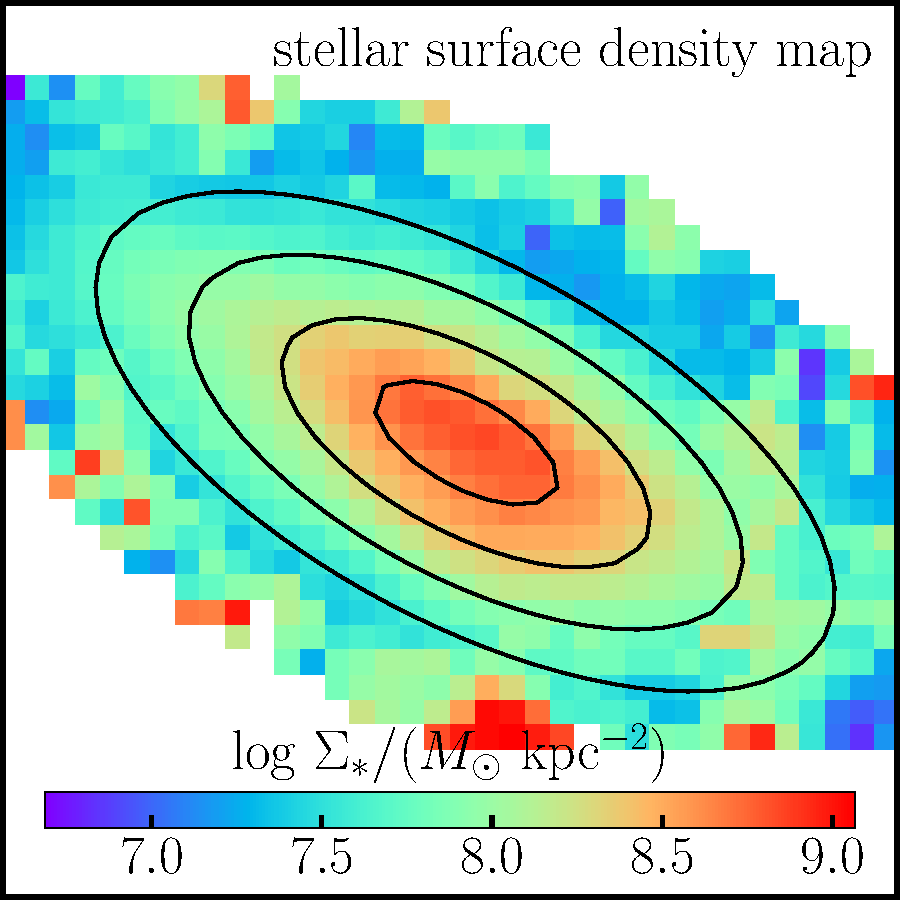
\includegraphics[width=.16\textwidth]{fig/physmap_lSDstar_ID03751.pdf}
    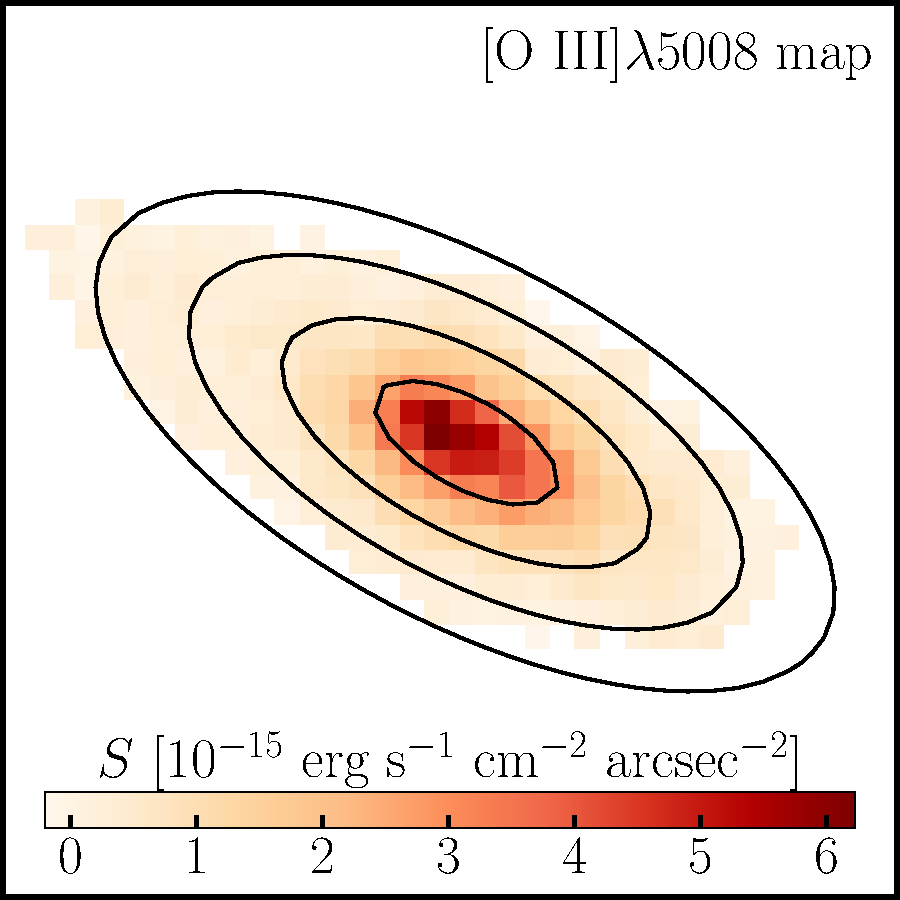
\includegraphics[width=.16\textwidth]{fig/combELmap_OIII_ID03751.pdf}
    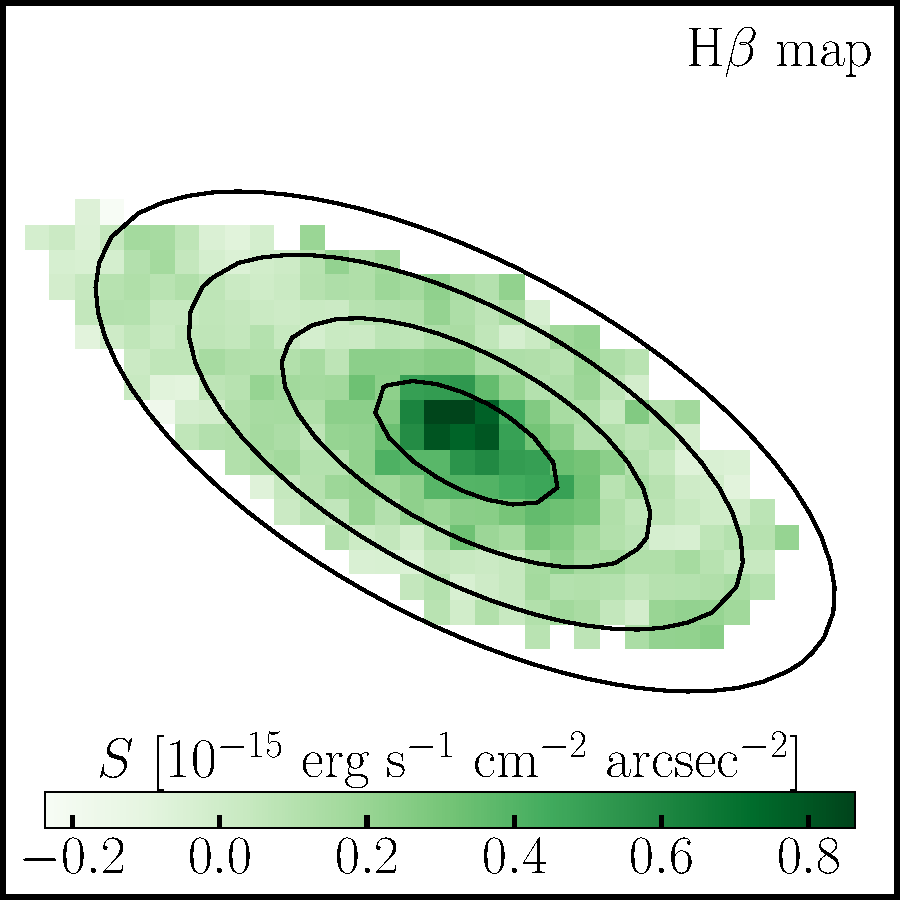
\includegraphics[width=.16\textwidth]{fig/combELmap_Hb_ID03751.pdf}
    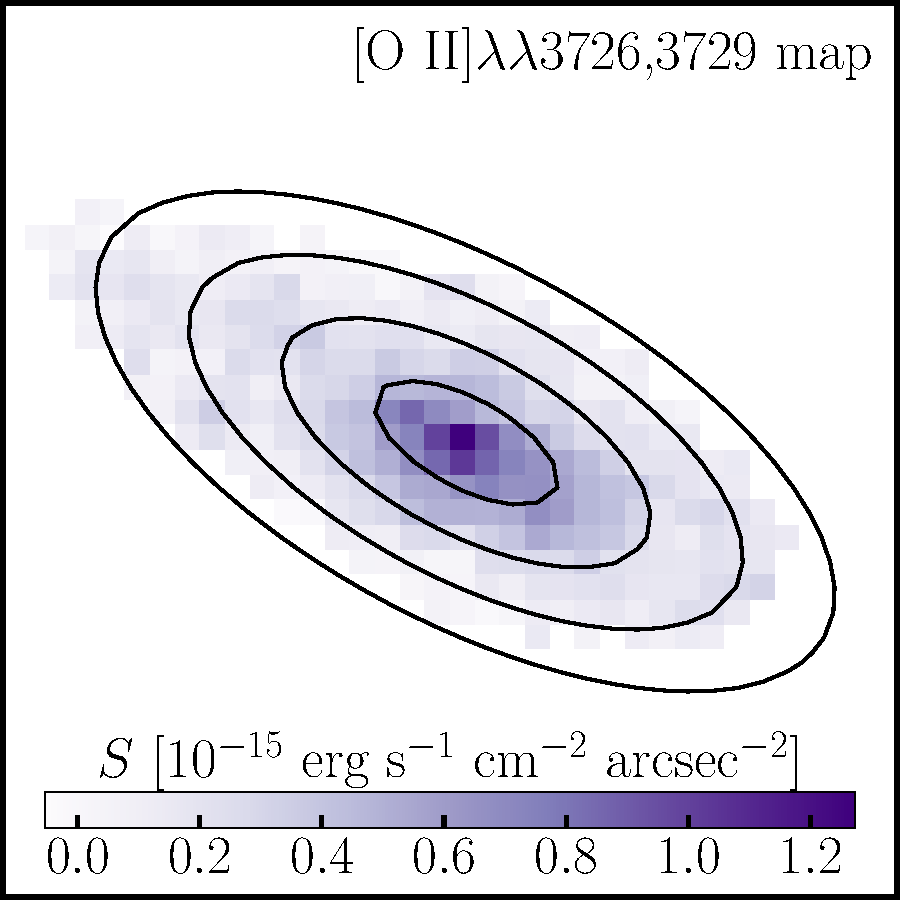
\includegraphics[width=.16\textwidth]{fig/combELmap_OII_ID03751.pdf}
    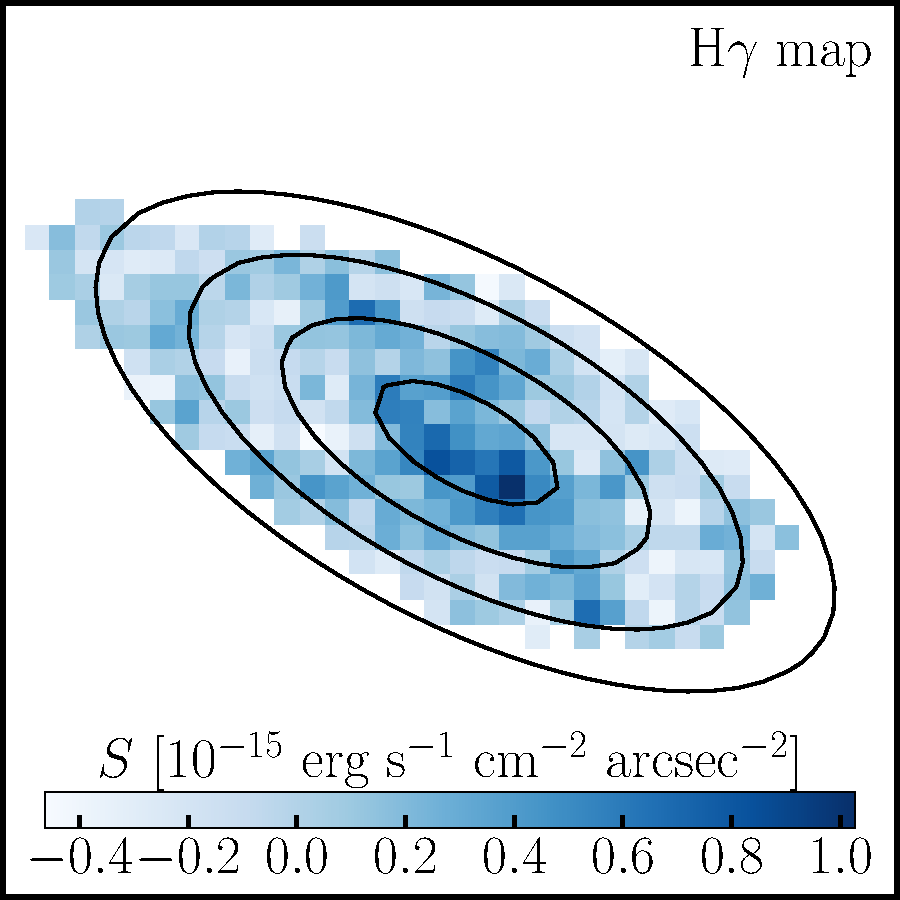
\includegraphics[width=.16\textwidth]{fig/combELmap_Hg_ID03751.pdf}\\
    \includegraphics[width=.16\textwidth]{fig/rgbstamp_ID01203.pdf}
    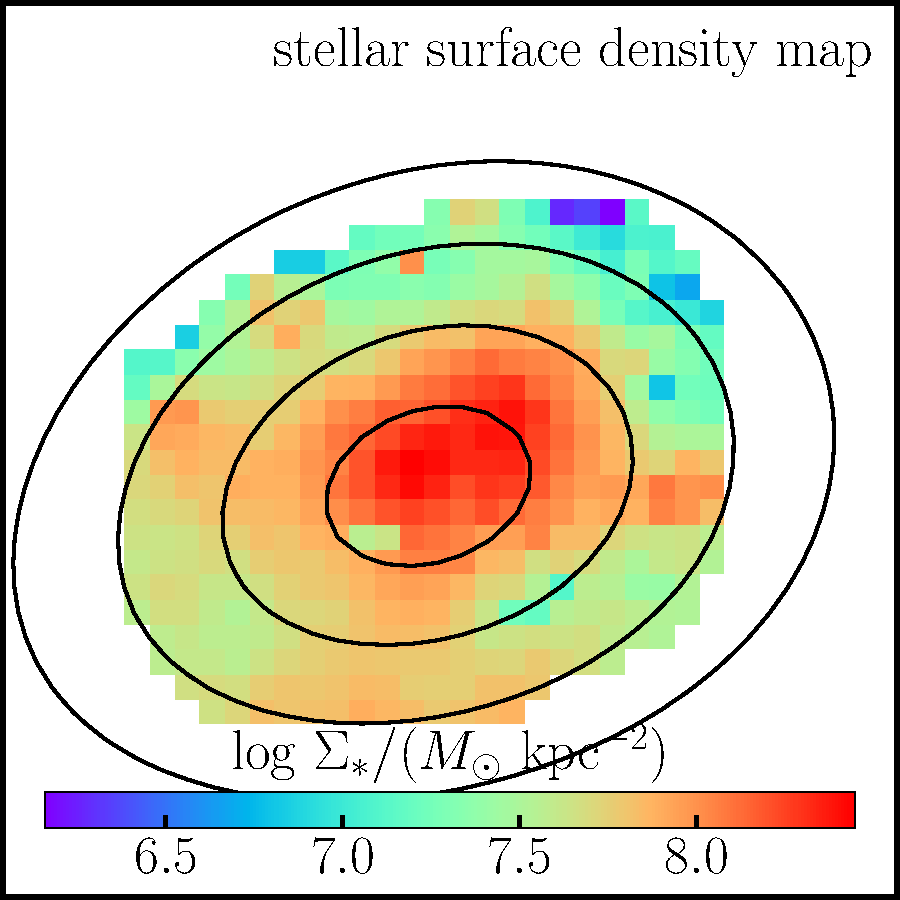
\includegraphics[width=.16\textwidth]{fig/physmap_lSDstar_ID01203.pdf}
    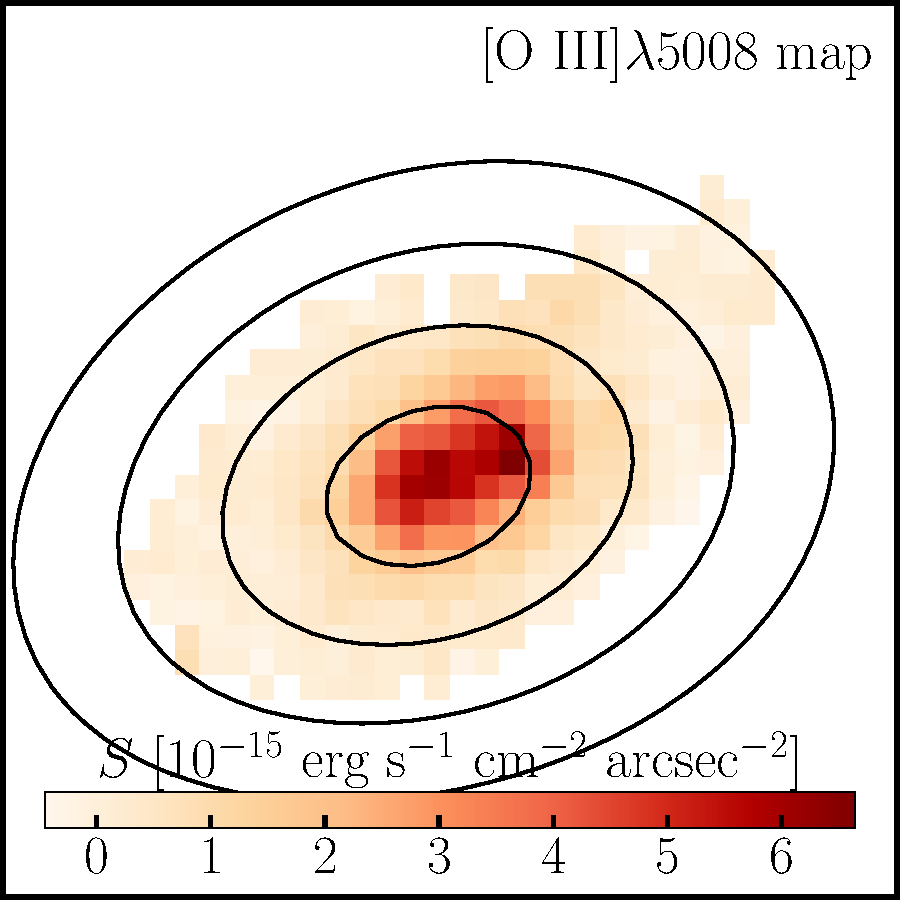
\includegraphics[width=.16\textwidth]{fig/combELmap_OIII_ID01203.pdf}
    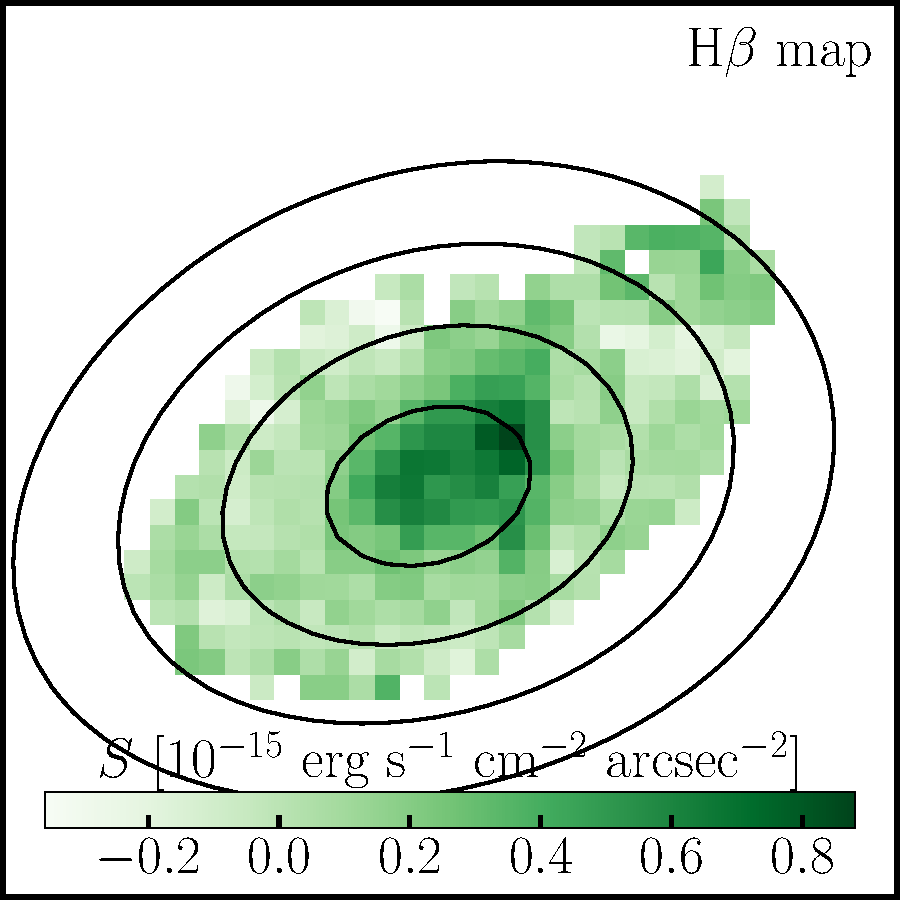
\includegraphics[width=.16\textwidth]{fig/combELmap_Hb_ID01203.pdf}
    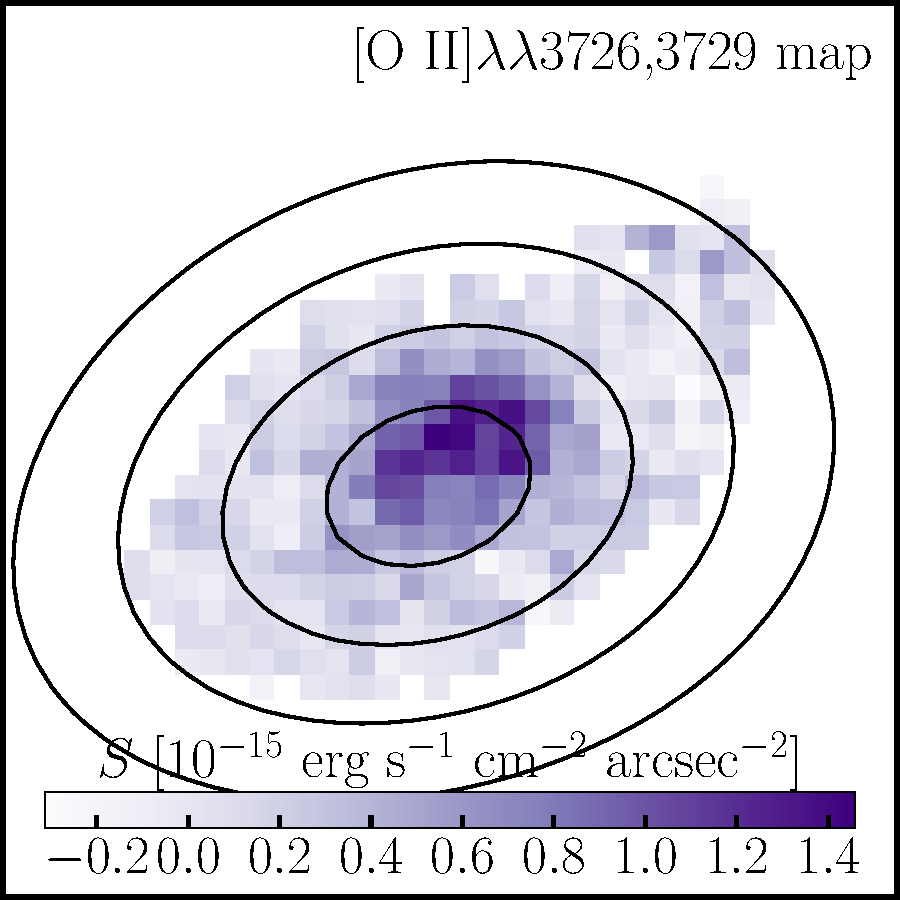
\includegraphics[width=.16\textwidth]{fig/combELmap_OII_ID01203.pdf}
    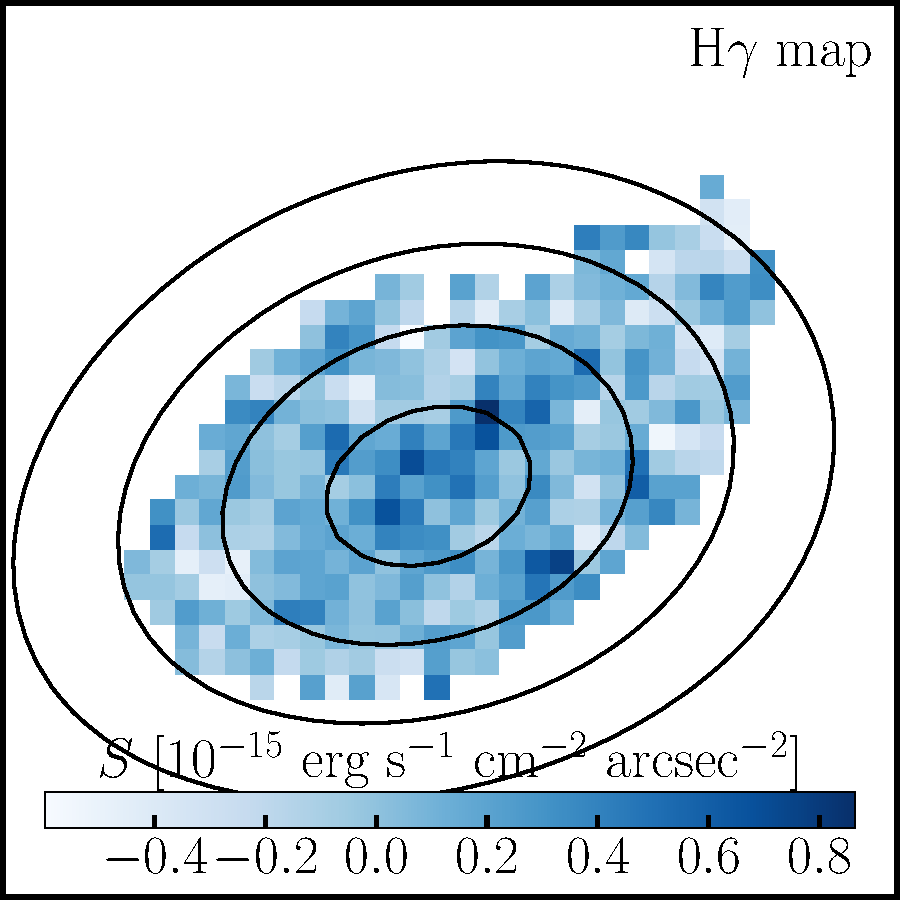
\includegraphics[width=.16\textwidth]{fig/combELmap_Hg_ID01203.pdf}
    \caption[Two star-forming dwarf galaxies at $z$$\sim$2 displaying unusually strong inverted metallicity gradients]{Two star-forming dwarf galaxies at $z$$\sim$2 displaying unusually strong inverted metallicity gradients, securely
    determined at sub-kpc spatial resolution. For each source we show, from left to right: color composite image (created from
    \hst broad-band photometry), stellar surface density map (obtained from SED fitting to \hst photometry), and surface
    brightness map of ELs \OIII, \Hb, \OII, and \Hg. The black contours overlaid represent the source plane de-projected
    galacto-centric radii with 1 kpc interval. The two light-dispersion directions for the grism exposures are 
    denoted by the orange and cyan arrows (see Figures~\ref{fig:3751spec} and \ref{fig:1203spec} for the 
    corresponding spectra).
    The spatial extent and orientation are unchanged for the two sources in all 2D
    stamps throughout. North is up and east is to the left.
    \label{fig:combELmap}}
\end{figure}
%= = = = = = = = = = = = = = = = = = = = = = = = = = = = = = = = = = = = = = = =

\section{Methods and Results}\label{sect:rslt}

In this section, we describe our key methods used to derive radial metallicity gradients (Section~\ref{sect:metalgrad}), 2D maps 
of \SFR, average stellar population age, and gas fraction (Section~\ref{sect:physprop}), as well as spatial 
distributions of net gaseous outflow rate and mass loading factor (Section~\ref{sect:regulator}).
The main results are presented alongside the corresponding methods.


\subsection{Radial Metallicity Gradients}\label{sect:metalgrad}

Since we infer metallicity from strong line flux ratio diagnostics, calibrated by either empirical methods, or 
theoretical methods, or a hybrid of both, it is essential to make sure that the line emission is not 
contaminated by active galactic nucleus (AGN) ionization or shock excitation.
As shown in Figure~\ref{fig:bluediagram}, we verify that our targets have a low probability (<\%10) of being 
classified as AGNs according to the mass-excitation diagram \citep{Juneau:2014ca}.
Their individual radial annuli also have excitation and ionization states, as revealed in their loci in the 
$f_{\OIII}/f_{\Hb}$ versus $f_{\OII}/f_{\Hb}$ diagram and the O$_{32}$(=$f_{\OIII}/f_{\OII}$) versus 
R$_{23}$(=$(f_{\OIII~5008} + f_{\OIII~4960} + f_{\OII})/f_{\Hb}$) diagram,
compatible with \HII regions \citep{Lamareille:2004jk,Rodrigues:2012dr,2015ApJ...813..126J}.
In the source ID 01203 covered by our follow-up \osiris observations (see Appendix~\ref{sect:kinem}), its 
integrated $f_{\NII}/f_{\Ha}$ ($\lesssim0.1$ at 3-$\sigma$) also shows no sign of AGN or shocked gas emission.

%= = = = = = = = = = = = = = = = = = = = = = = = = = = = = = = = = = = = = = = =
%%% Figures
\begin{figure}
    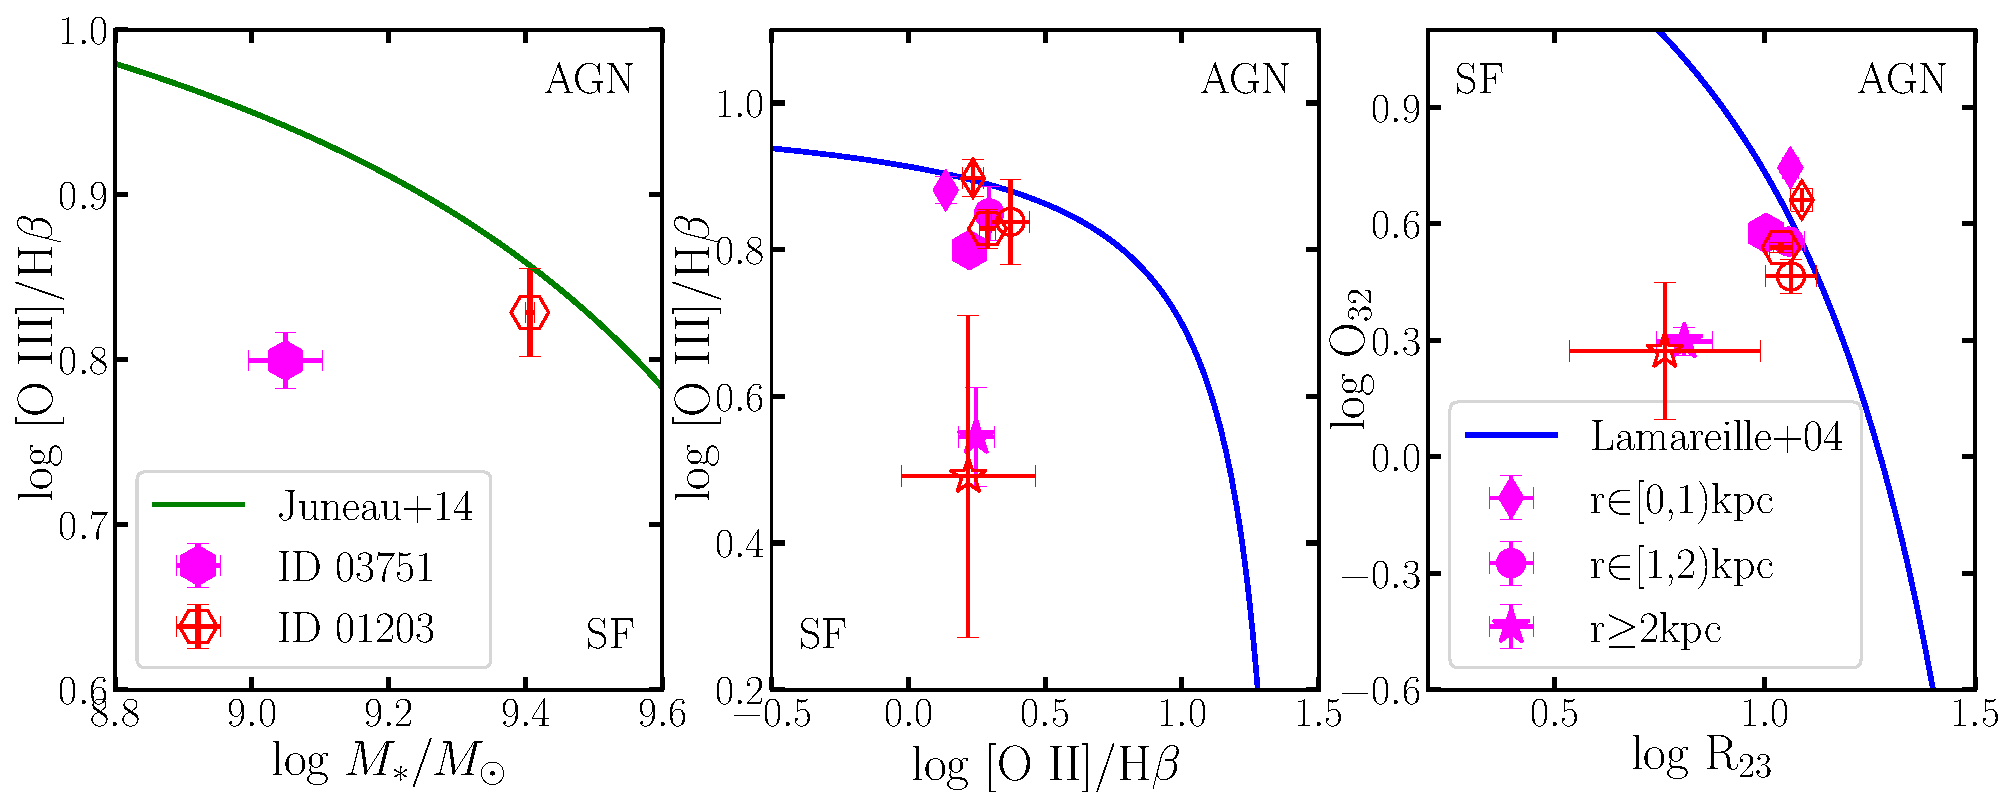
\includegraphics[width=\textwidth]{fig/bluediagram.pdf}
    \caption[The diagnostic diagrams for our sources.]{The diagnostic diagrams for our sources.
    On the left, we show the mass-excitation diagram
    with the demarcation scheme between the loci of AGNs and 
    star-forming (SF) galaxies proposed in \citet{Juneau:2014ca}. Our galaxies can be safely classified as the 
    latter.
    In the middle and right panels, we show the ``blue'' diagrams with the boundaries described by \citet{Lamareille:2004jk}.
    Following the conventions in the left panel, we use filled symbols to represent measurements for ID 03751 
    whilst empty ones for ID 01203.
    Furthermore, the hexagons correspond to the measurements integrated over the entire galaxies (as in the left 
    panel), whereas the other symbols denote results obtained in different radial annuli, as explained in the 
    legend of the right panel.
    Again we see that the contamination from AGN ionization is minimum for our sources, even in the central 
    regions.
    The two galaxies presented in this work share similar evolutionary trends in their excitation and ionization 
    states with respect to galacto-centric radius, in addition to the strongly inverted radial gradient in 
    metallicity (see Figure~\ref{fig:oh12grad}).
    \label{fig:bluediagram}}
\end{figure}
%= = = = = = = = = = = = = = = = = = = = = = = = = = = = = = = = = = = = = = = =

Our measurements of radial \mgs largely follow the procedures described in our previous work \citep{Wang:2016um}.
We use a Bayesian approach to jointly infer metallicity (\oh), nebular dust extinction ($\Av^{\rm N}$), and de-reddened \Hb flux
($f_{\Hb}$).  We explore the parameter space using the Markov Chain Monte Carlo sampler \emc\citep{ForemanMackey:2013io}.
The likelihood function is given by $\mathrm{L}\propto\exp(-\chisq/2)$ with
\begin{align}
    \chisq = \sum_i \frac{\(f_{\el{i}} - R_i \cdot f_{\Hb}\)^2}
        {\(\sigma_{\el{i}}\)^2 + \(f_{\Hb}\)^2\cdot\(\sigma_{R_i}\)^2},
\end{align}
where \el{i} corresponds to each available EL: \OIII, \Hb, \OII, and \Hg. $f_{\el{i}}$ and $\sigma_{\el{i}}$ are the flux and uncertainty of \el{i}. $R_i$ is the flux ratio between \el{i} and \Hb, with $\sigma_{R_i}$ being the intrinsic scatter at fixed physical properties.
In the case $\el{i}=\Hg$, $R_i$ is given by the Balmer decrement $f_{\Hg}/f_{\Hb}=0.47$.
For $\el{i} \in \{\OII,~\OIII\}$, $R_i$ and $\sigma_{R_i}$ are given by the strong line metallicity diagnostics 
($f_{\OIII}/f_{\Hb}$ and $f_{\OII}/f_{\Hb}$) calibrated by \citet{2008A&A...488..463M}.
The \citet{2008A&A...488..463M} calibrations combine the direct electron temperature measurements from the Sloan 
Digital Sky Survey in the low-metallicity (\oh<8.35) branch \citep{2006A&A...459...85N} and the photoionization 
model predictions in the high-metallicity (\oh>8.35) branch \citep{Kewley:2002ep}, providing a continuous and 
coherent recipe over a wide metallicity range.
We also adopt the empirical calibrations by \citet{Curti:2016fn} based on metallicities given by pure electron
temperature method, and verified that there is no significant change in our gradient measurements.
The same process is applied to both galaxy-integrated fluxes and to fluxes measured at individual spatial pixels 
(spaxels).


To obtain the correct intrinsic de-projected distance scale for each spaxel, we conducted full source plane morphological
reconstruction of our sources.
%Since our targets are gravitationally lensed, we must account for lensing magnification to determine their true morphologies and
%global properties. We note that surface densities and flux ratios (used to determine metallicity) are unaffected by
%lensing.
We ray-trace the image of each galaxy to its source plane using up-to-date lens models for each cluster: the macroscopic
model of \SJ version 4 for \clsan \citep{Johnson:2014cf}, and the \textsc{Zitrin} version 2 model for \clba
\citep{2015ApJ...801...44Z}. Other lens models are available for these clusters 
\cite[\eg][]{Diego:2016ww,Strait:2018ul} and we verified that the morphology of each source
is robust to the choice of model.

For each source, we fit the SED of individual spaxels using the procedures described in Section~\ref{sect:data}, 
obtaining the 2D stellar surface density (\Sstar) map shown in Figure~\ref{fig:combELmap}. Then we reconstruct 
\Sstar map in the source plane by de-lensing the surface densities according to the deflection field given by the 
macroscopic lens models.
To minimize the stochasticity in stellar population synthesis \citep{Fouesneau:2010ea,Eldridge:2012ds}, 
we make sure that the source plane resolution elements during this reconstruction contain enough stellar masses 
($\gtrsim 10^5$ \Msun) to be representative of complete stellar populations.
The axis ratios, inclinations, and major axis orientations are determined from an elliptical Gaussian fit. This 
procedure provides the intrinsic lensing-corrected morphology, and in particular, the galacto-centric radius at 
each point of the observed images.
The radial scale as black contours in all figures is used to establish the absolute metallicity gradient slope (i.e., in units of 
dex per proper kpc).
From the source reconstructed morphology, we measure their effective radius where the enclosed mass 
reaches half the total mass of the source. The measurements are represented by $R_{\rm eff}$ in 
Table~\ref{tab:srcprop}.

Figure~\ref{fig:oh12grad} shows the 2D maps of metallicity of our selected two dwarf galaxies at $z\sim2$.
Clearly, the outskirts of our galaxies display highly elevated oxygen abundance ratios.
In particular, the outskirts of ID 03751 are more metal enriched by $\sim$0.4 dex (\ie a factor of 2.5) than its center, and more 
metal-rich by $\sim$0.2 dex than the value inferred based on the fundamental metallicity relation (FMR) given its 
integrated \Mstar \cite{2010MNRAS.408.2115M,Mannucci:2011be}.
Note that our metallicity measurements extend beyond the source effective radius to cover large enough 
dynamic range, but not into the region where a plateau/flattening in metallicity \citep[\ie, at $R>2-2.5 R_{\rm 
eff}$,][]{2014A&A...563A..49S,SanchezMenguiano:2016gj,Molla:2018em} is likely to occur, which might bias the 
overall gradient determination.
For the first time, we are able to detect strongly inverted metallicity gradients in $z$$\sim$2 dwarf galaxies
at unprecedentedly high confidence: 0.122$\pm$0.008 dex/kpc for ID 03751 ($\sim15.2\sigma$), and
0.111$\pm$0.017 dex/kpc for ID 01203 ($\sim6.5\sigma$).

The question is thus what caused these dwarf galaxies to have such strongly inverted gradients?
First of all, our sources show no evidence of major mergers, supported by their regular morphology displayed in the 2D maps of 
\Mstar and EL surface brightness in Figure~\ref{fig:combELmap}.
For source ID 01203 with \osiris data, this statement is further strengthened by the kinematic evidence of disk orderly rotation.
Secondly, the fact that the outskirts of our sources show elevated metallicity as compared to the FMR 
expectations indicates that there are more metals in the outer regions than could be produced by the stars in those 
regions.
This discourages any explanations involving solely low-metallicity gas inflows, not limited to those induced by mergers.
In the subsequent sections, we thus gather all available pieces of observational evidence to further investigate the possible 
cause.

%= = = = = = = = = = = = = = = = = = = = = = = = = = = = = = = = = = = = = = = =
%%% Figures
\begin{figure}
    \centering
    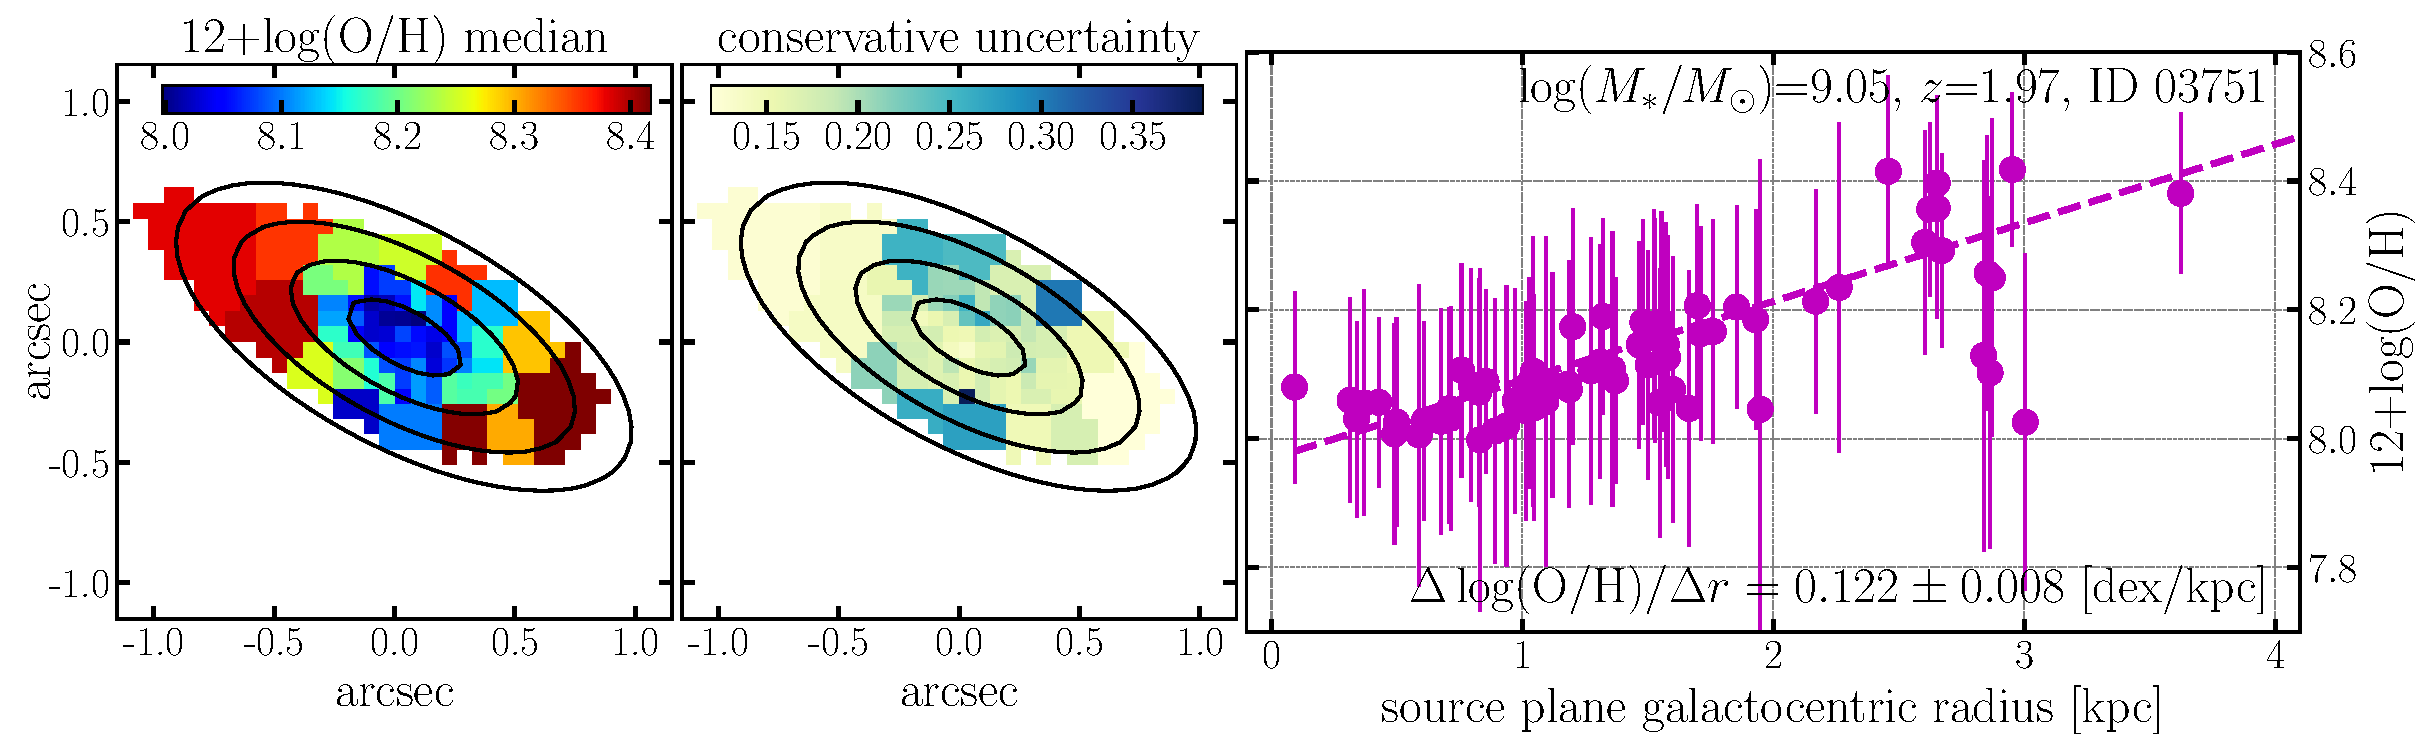
\includegraphics[width=\textwidth]{fig/metalgrad_ID03751.pdf}\\
    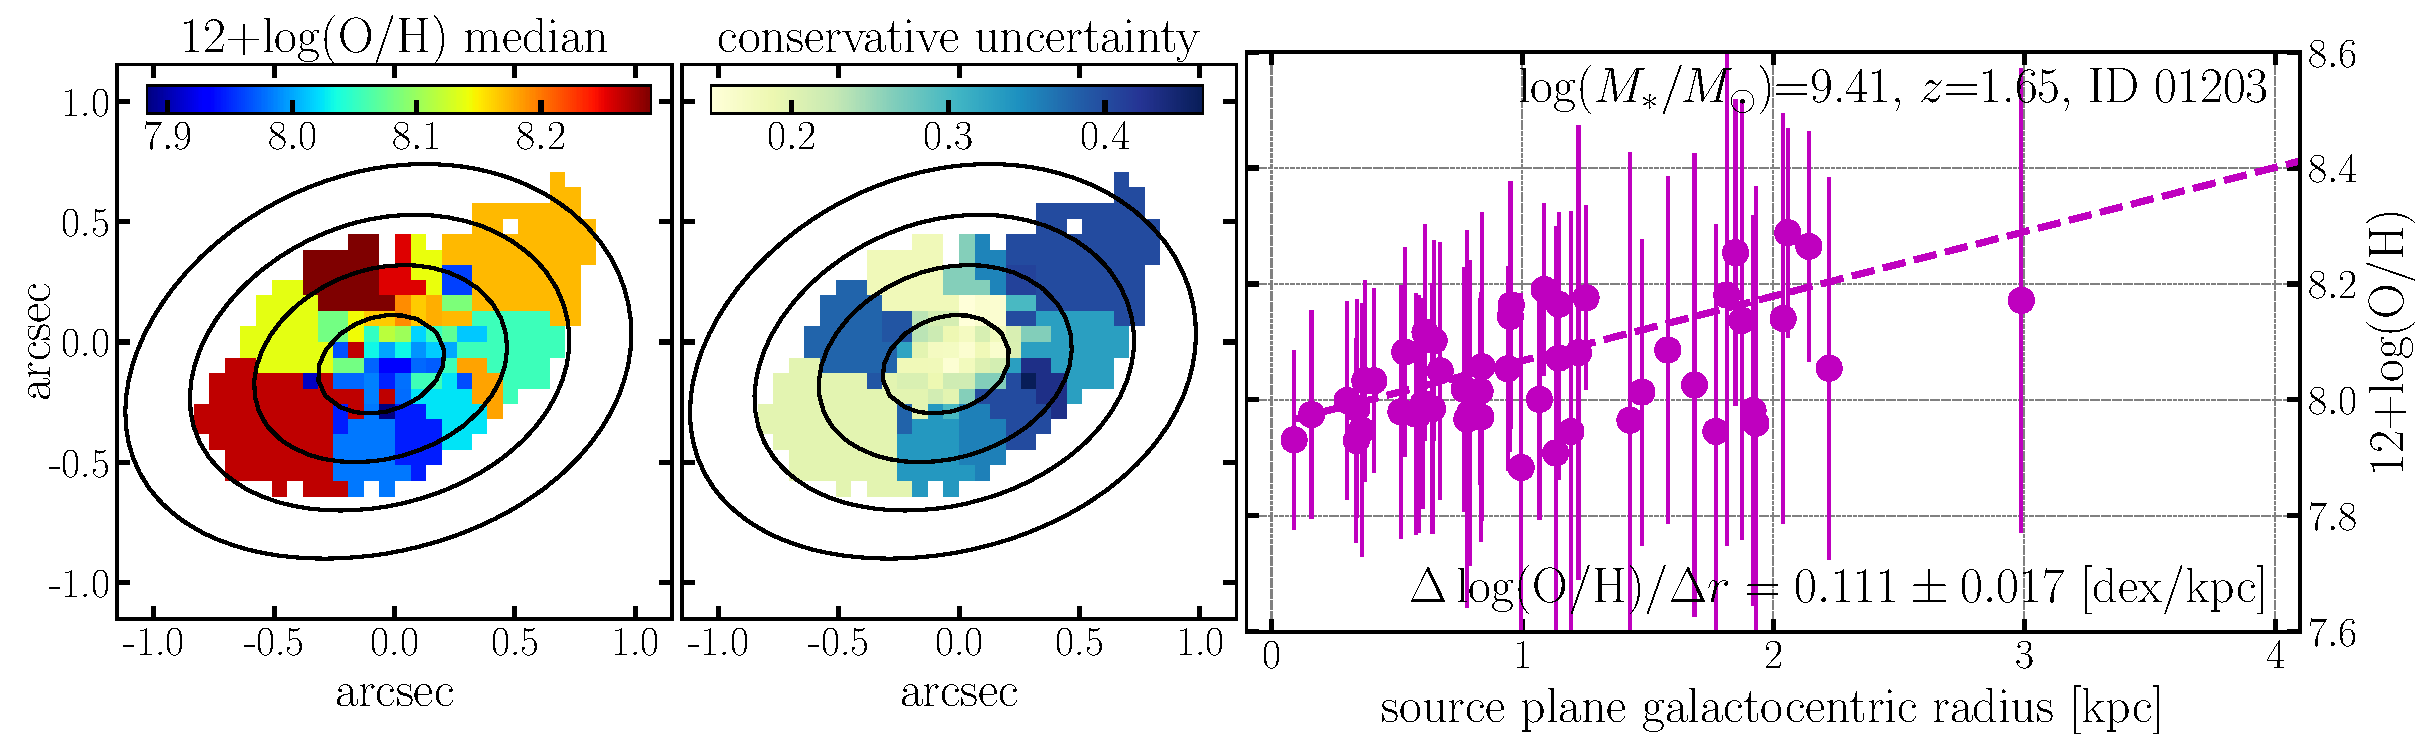
\includegraphics[width=\textwidth]{fig/metalgrad_ID01203.pdf}
    \caption[Metallicity maps and radial gradient measurements of the two galaxies.]
    {Metallicity maps and radial gradient measurements of the two galaxies. The left panels show the 2D maps of the median
    value estimates of metallicity, and the central panels show their conservative uncertainties (\ie the larger side of the
    asymmetric 1-$\sigma$ error bars). The right panels show the corresponding radial gradients measurements.
    The black contours again mark the source plane de-projected galacto-centric distances as in 
    Figure~\ref{fig:combELmap}.
    We adopted weighted Voronoi tessellation \citep{Cappellari:2003eu,Diehl:2006cz},
    with a SNR of 10 on \OIII for the binned metallicity maps.
    In the right column, these bins are plotted as individual data points.
    The dashed line denotes the linear regression from these points, with the measured radial slope shown at the bottom of each
    panel.  For both galaxies, the radial gradient is strongly positive (\ie inverted).
    \label{fig:oh12grad}}
\end{figure}
%= = = = = = = = = = = = = = = = = = = = = = = = = = = = = = = = = = = = = = = =


\subsection{\SFR, Stellar Population Age, and Gas Fraction}\label{sect:physprop}

To understand the cause of the strongly inverted metallicity gradients seen in these dwarf galaxies,
we combine their EL maps with \hst broad-band photometry to derive 2D maps of \Mstar, \SFR,
stellar population age, and gas surface density for each galaxy.
The \SFR is derived from extinction-corrected Balmer emission line flux. Maps of \Hb and \Hg emission are shown in
Figure~\ref{fig:combELmap}. The \Hb/\Hg line ratio provides a measurement of nebular extinction although it is limited by the
modest signal-to-noise of \Hg. We obtain more precise results from \hst photometry, by converting \B-\I color maps to spatial
distributions of stellar reddening $E_{\rm S}(B-V)$ \citep{Daddi:2004hj}. Nebular reddening $E_{\rm N}(B-V)$ is then calculated
following \citet{Valentino:2017by}.  The nebular reddening maps of both our galaxies show lower dust attenuation in centers than
that in outskirts, consistent with the inverted metallicity gradients shown in Figure~\ref{fig:oh12grad}.

We calculate extinction in \Hb adopting a \citet{1989ApJ...345..245C} dust extinction law
(with \Rv=3.1) and assuming Case B recombination with Balmer ratios appropriate for fiducial \HII region properties (\ie,
\Ha/\Hb~=~2.86).  Finally, we convert intrinsic \Ha luminosity to \SFR through the commonly used calibration
\citep{Kennicutt:1998ki},
\begin{align}
    {\rm SFR} = 4.6\times10^{-42}~ \frac{L(\Ha)}{\rm erg/s} \quad [\Msun/\textrm{yr}],
\end{align}
appropriate for the \citet{Chabrier:2003ki} IMF.
This provides the instantaneous star formation rate on $\sim$10 Myr time scales; we note that the ultraviolet continuum probed by
\hst photometry is sensitive to recent \SFR over a longer time span ($\sim$100-300 \Myr). The short timescales probed by Balmer
emission are most relevant for determining outflow physical properties, which are highly dynamic on small spatial scales, \eg, at 
sub-kpc level.
%($v_{\rm wind}\gtrsim v_{\rm circ}$, $<1$ \kpc scales).

Next we derive average stellar age maps, using the spatial distribution of EL EW as the primary constraint. We
calculate \Hb rest-frame EWs from our maps of the emission line flux and stellar continuum flux density. Stellar continuum maps
are corrected for emission line contamination as described in Section~\ref{sect:data}. We correct for stellar Balmer absorption
which we estimate to be rest-frame EW~$\sim$3 \AA\ in \Hb based on the derived galaxy properties \citep{Kashino:2013ev}.  Maps of
\Hb EW are then converted to average stellar age using a series of \burst stellar population synthesis
models \citep{Leitherer:1999jt,Zanella:2015ej} assuming 1/5 solar metallicity and constant star formation history.

We also compare the age estimates given by our SED fitting (Section~\ref{sect:data}) and \Hb rest-frame EW using the method
described above. The median values given by the former practice are systematically larger than those of the latter by $\sim$0.5
dex, but we note that the uncertainties by the SED fitting are usually much larger due to the absence of prominent continuum
spectral age indicators, \eg, \Dn and \HdA \citep{Kauffmann:2003cu}. Hence, we adopt the results from \Hb rest-frame EW as the
average age for stellar populations throughout our analysis, as we consider this a more reliable estimate.

Finally, we calculate the gas fraction defined as
\begin{align}
    \fgas=\Sgas/\left(\Sgas+\Sstar\right).
    \label{eq:fgas}
\end{align}
Since we do not directly observe the bulk of interstellar gas, we instead estimate gas surface density \Sgas by 
inverting the
Kennicutt-Schmidt (KS) law \citep{Schmidt:1959bp,Kennicutt:1998id}, \ie, $\Sigma_{\SFR}\propto\Sgas^{N}$ together with our
measurements of $\Sigma_{\SFR}$ described above.  We adopt the more robust extended version of the KS law developed by 
\citet{Shi:2011ck,Shi:2018wf} which is especially useful in low density regimes:
\begin{align}
    \frac{\Sigma_{\SFR}}{\Msun/\yr/\kpc^2} = 10^{-4.76} \left(\frac{\Sstar}{\Msun/\pc^2}\right)^{0.545}
    \left(\frac{\Sgas}{\Msun/\pc^2}\right)^{1.09}.
    \label{eq:KSlaw}
\end{align}
This extended KS law has been tested in numerous ensembles of galaxies as well as low surface brightness regions in individual
galaxies, and is shown to have relatively small scatter ($\sim$0.3 dex) over a large dynamic range of gas and \SFR surface
densities. We have combined in quadrature this systematic uncertainty of 0.3 dex in our estimates of \Sgas.

Figure~\ref{fig:physmap} shows the derived 2D maps of \SFR, average stellar age, and gas fraction.
In general, we observe centrally concentrated star formation, with the most actively star-forming regions having surface densities 
$\gtrsim10~\Msun/\yr/\kpc$.
On average, the central regions also have older stellar populations and smaller gas fractions than the outskirts, indicating that
the outer regions are still in the early stages of converting their gas into stars.
These features together indicate that we are witnessing the rapid build-up of galactic disks through in-situ star formation and 
strongly support an inside-out mode of galaxy growth \citep{Nelson:2014is,2013ApJ...765...48J}.

%= = = = = = = = = = = = = = = = = = = = = = = = = = = = = = = = = = = = = = = =
%%% Figure:
\begin{figure}
    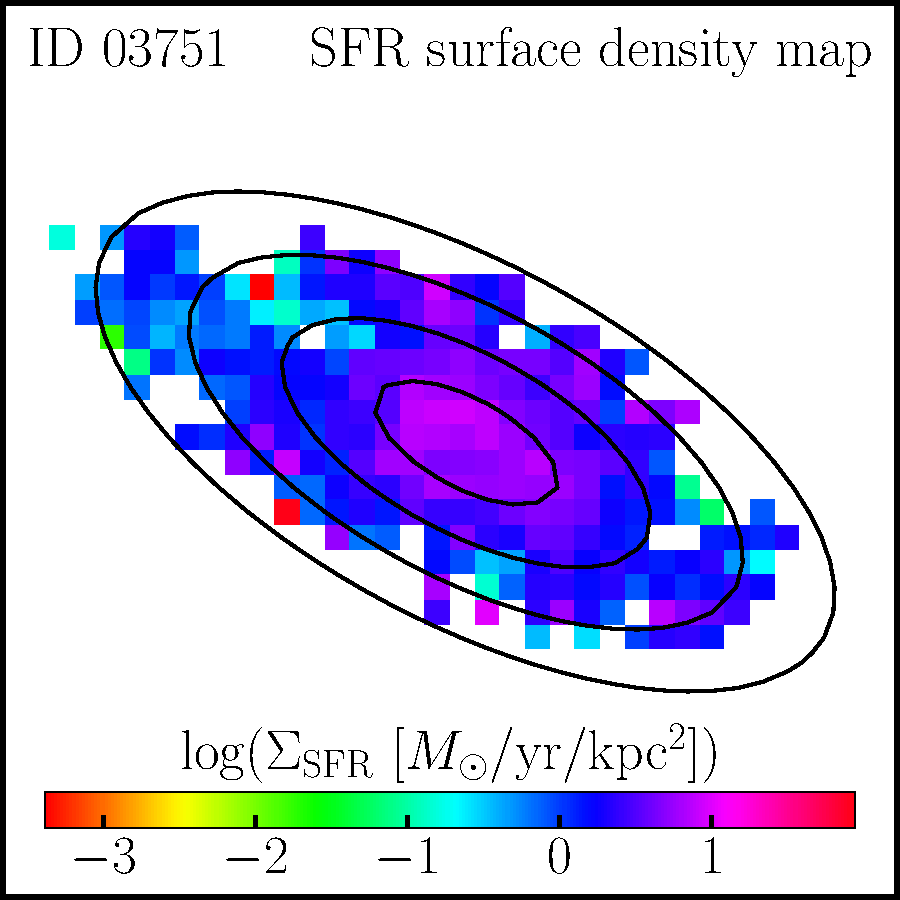
\includegraphics[width=.33\textwidth]{fig/physmap_lsfr_ID03751.pdf}
    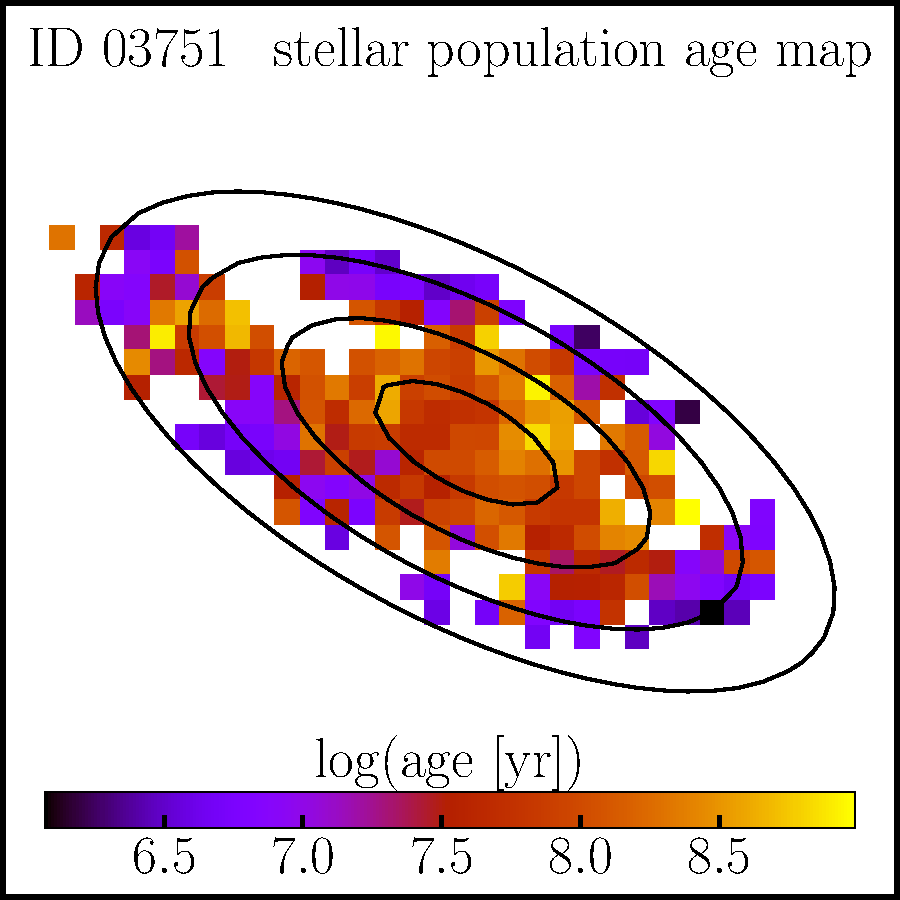
\includegraphics[width=.33\textwidth]{fig/physmap_lage_ID03751.pdf}
    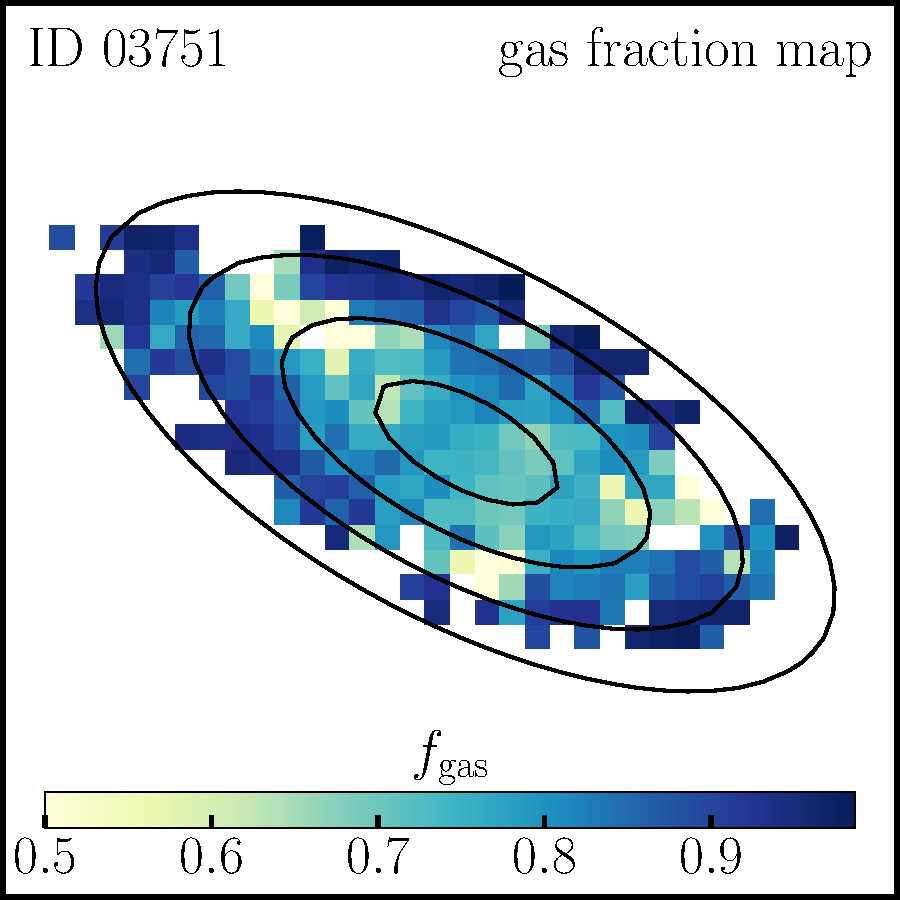
\includegraphics[width=.33\textwidth]{fig/physmap_fgas_ID03751.pdf}\\
    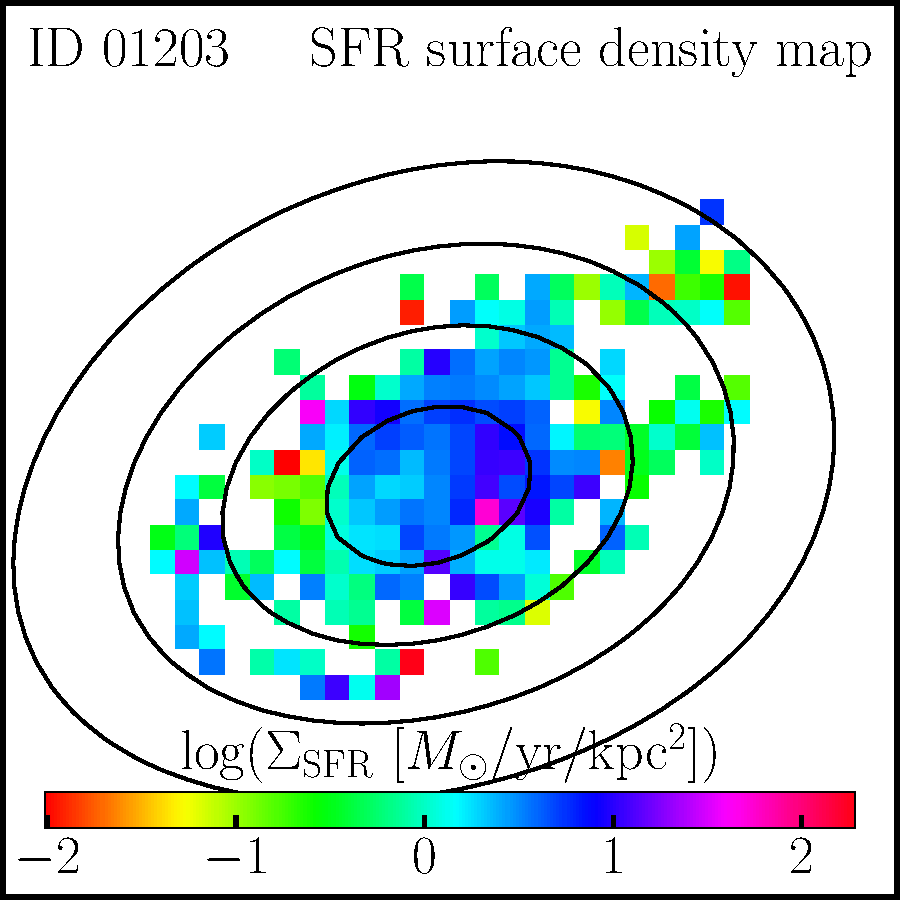
\includegraphics[width=.33\textwidth]{fig/physmap_lsfr_ID01203.pdf}
    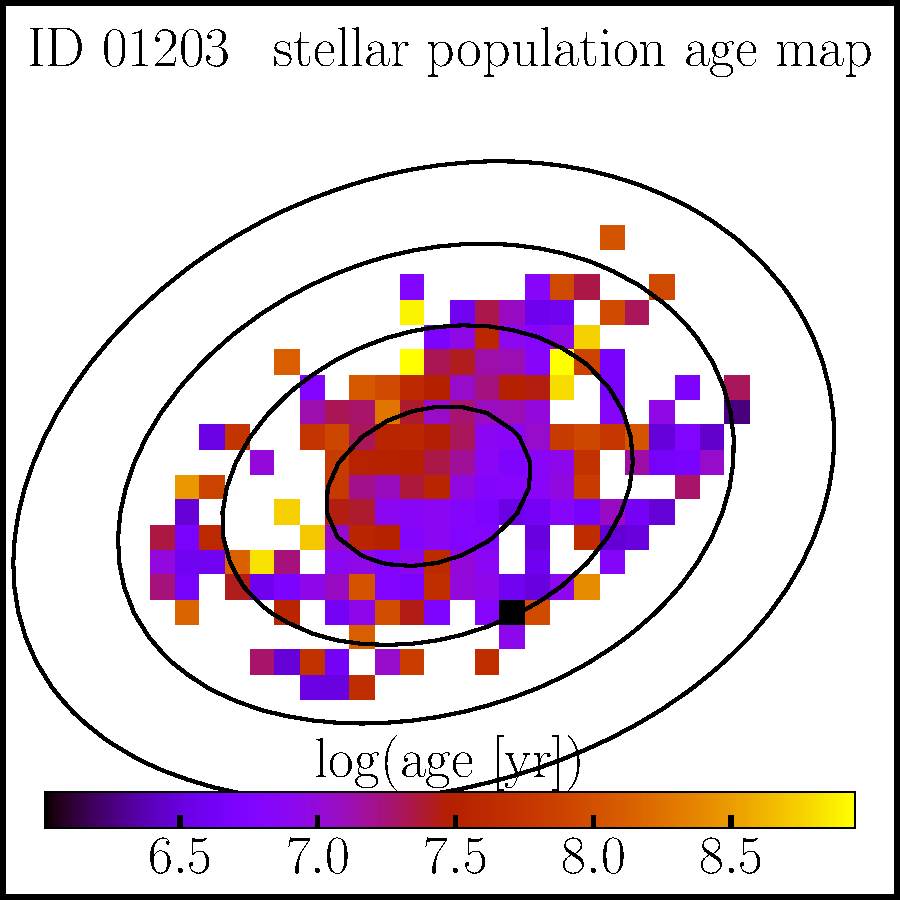
\includegraphics[width=.33\textwidth]{fig/physmap_lage_ID01203.pdf}
    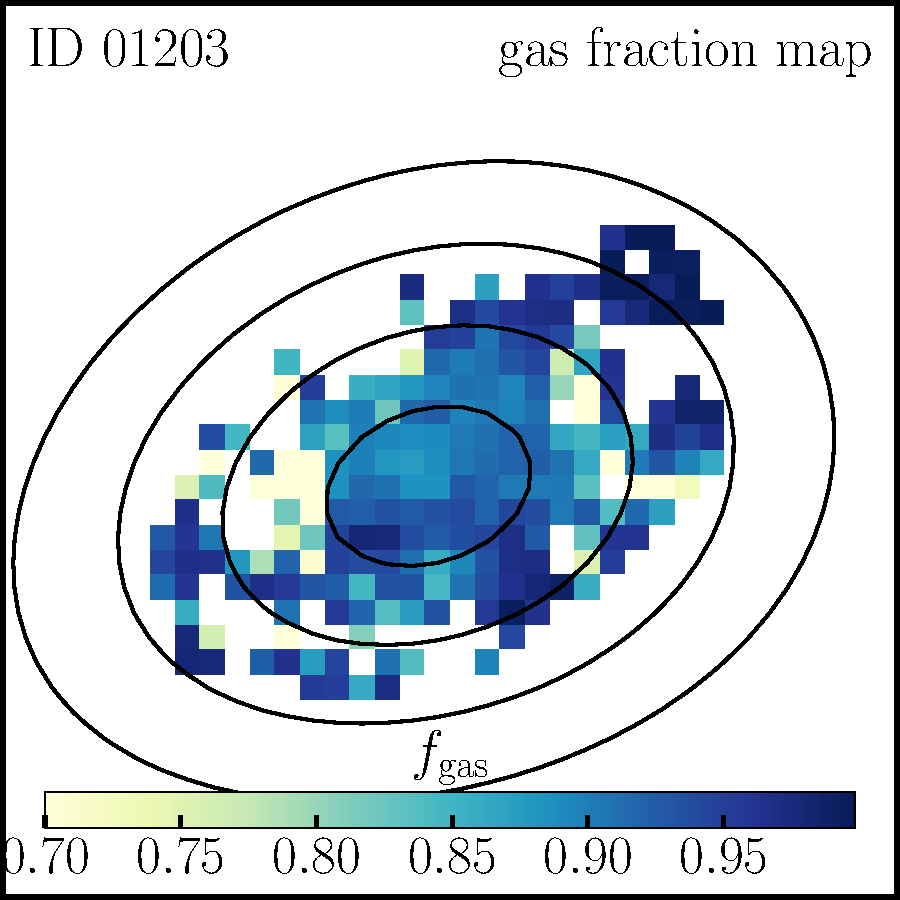
\includegraphics[width=.33\textwidth]{fig/physmap_fgas_ID01203.pdf}
    \caption[Maps of SFR surface density, average stellar population age, and gas fraction for our galaxies,
    derived from our spatially resolved analysis of stellar continuum and nebular emission.]
    {Maps of SFR surface density, average stellar population age, and gas fraction for our galaxies, derived from our
    spatially resolved analysis of stellar continuum and nebular emission.
    The spatial extent and orientation follows that in Figure~\ref{fig:combELmap}.
    We see that for both sources compared with their outskirts, their central regions have more active star formation, older 
    stellar population, and lower gas fraction.
    \label{fig:physmap}}
\end{figure}
%= = = = = = = = = = = = = = = = = = = = = = = = = = = = = = = = = = = = = = = =

As in \citet{Cresci:2010hr}, we compare our radially averaged \fgas and metallicity measurements against the predictions from
the simple chemical evolution model developed by \citet{Erb:2008di}.
To separate the effects of gas inflows and outflows, we compute two extreme sets of models, one being pure gas 
accretion (\ie with no outflows, $f_o=\Psi/\SFR=0$) and the other corresponding to the leaky box model (\ie with 
no inflows, $f_i=\Phi/\SFR=0$).
The results are shown in Figure~\ref{fig:Zerb_fgas}.
We note that for the pure gas accretion scenario, \fgas cannot decrease beyond a certain value, \ie,
$$
    \fgas^{\rm min} = 1-\frac{1-R}{f_i - f_o}
$$
where $f_o=0$ and $R$ is the instantaneous return fraction. This $\fgas^{\rm min}$, implicitly imposed by Eq.~(11) of 
\citet{Erb:2008di}, physically indicates that galaxies cannot exhaust their gas reservoir to below a certain amount without the 
help of outflows,
under the equilibrium condition with steady gas accretion (see Section~\ref{sect:regulator} when this equilibrium assumption is 
relaxed).
Therefore, the pure gas accretion scenario cannot explain the observed gas fractions in our source central regions (at $\lesssim$ 
2\kpc) where metallicities are also lower.
The leaky box model, on the other hand, provides a plausible explanation for our observation such that the outflow rate tends to 
increase towards galaxy center.
However, we stress that in reality both gas outflows and inflows are acting together to re-distribute 
metallicity. This test using simple chemical evolution models just clearly shows that using gas accretions 
\emph{alone} cannot explain our spatially resolved measurements.

%= = = = = = = = = = = = = = = = = = = = = = = = = = = = = = = = = = = = = = = =
%%% Figure:
\begin{figure}
    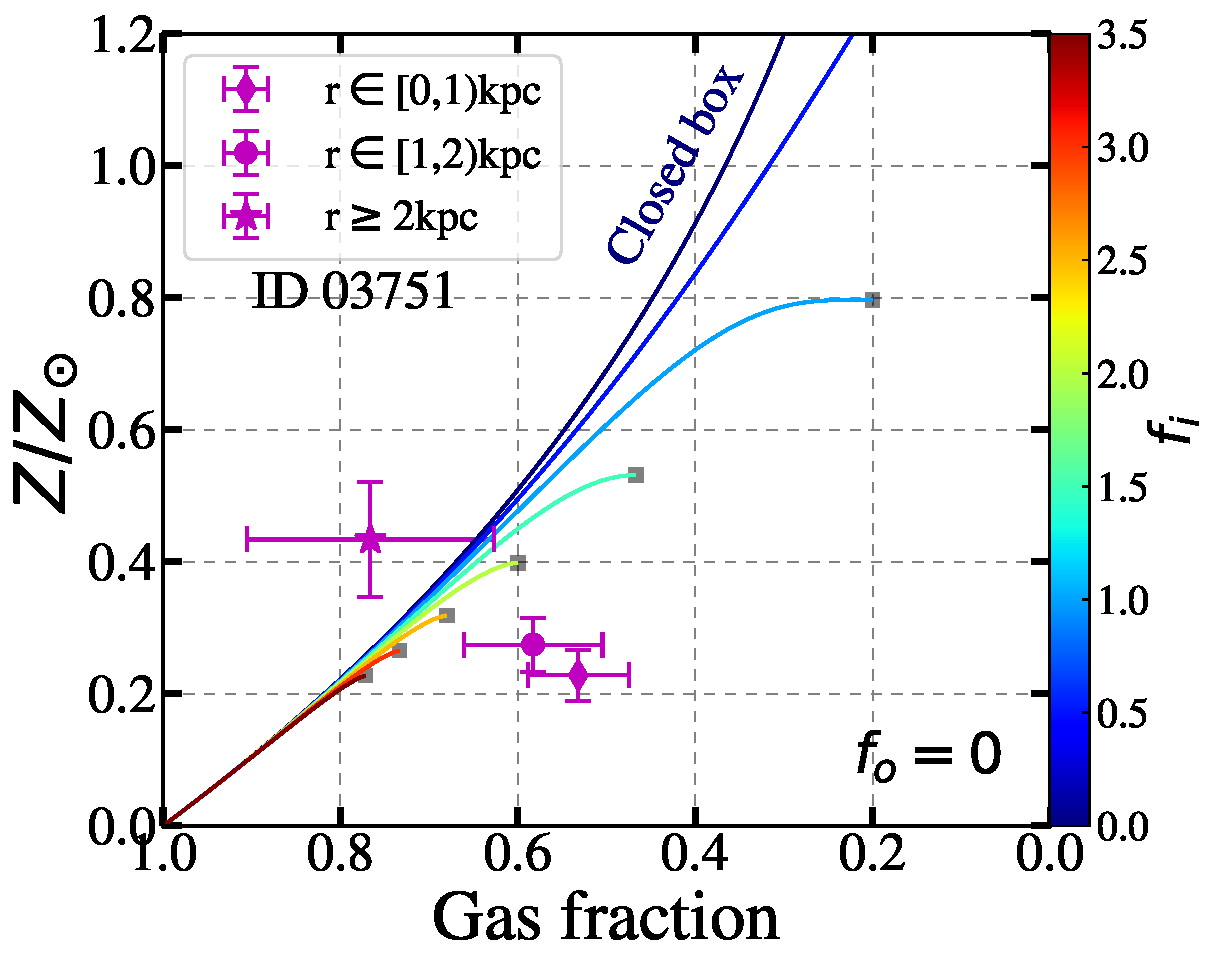
\includegraphics[width=.5\textwidth]{fig/Zerb_fgas_fixf_o.pdf}
    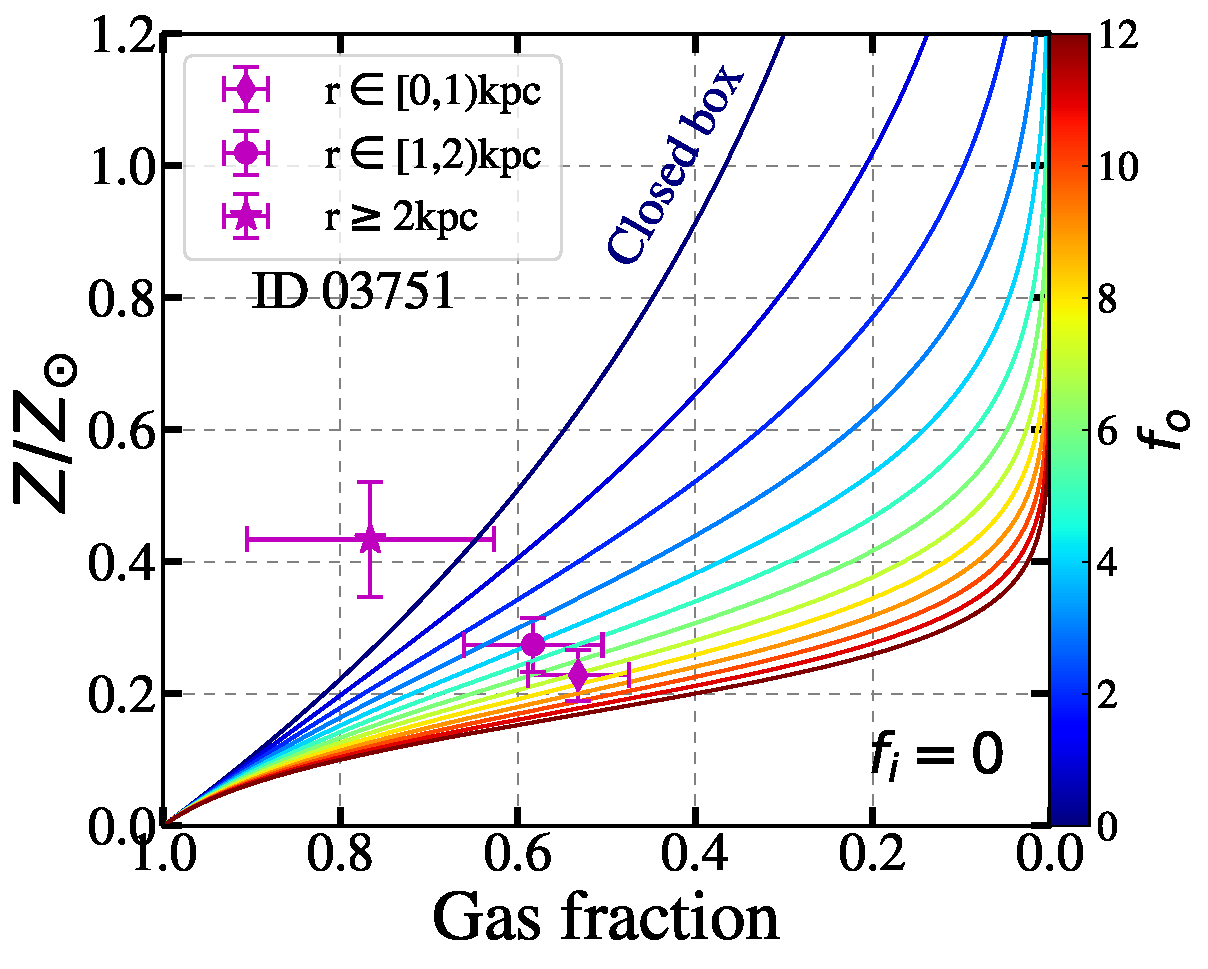
\includegraphics[width=.5\textwidth]{fig/Zerb_fgas_fixf_i.pdf}
    \caption[Gas fraction and metallicity estimated in different radial annuli.]
    {Gas fraction and metallicity estimated in different radial annuli for galaxy ID 03751.
    The diamond, circle, and star symbols represent measurements derived at a galacto-centric radius of $r\in[0,1)$\kpc,
    $r\in[1,2)$\kpc, and $r\gtrsim2$\kpc, respectively.
    We also overlay the curves calculated from a simple chemical evolution model \cite{Erb:2008di} under extreme conditions, \ie,
    pure gas inflow ($f_o=0$; left) and pure gas outflow ($f_i=0$; right).
    Note that the trajectories of pure gas inflow cases cease at the grey squares for high infall rate ($f_i\gtrsim1$) conditions;
    any extensions from those grey squares toward low gas fraction (while fixing metallicity) are unphysical.
    This simple comparison shows that purely gas accretion does not suffice to explain the strong inverted gradients seen in our
    galaxies.
    \label{fig:Zerb_fgas}}
\end{figure}
%= = = = = = = = = = = = = = = = = = = = = = = = = = = = = = = = = = = = = = = =

\subsection{Spatially Resolved Gaseous Outflows}\label{sect:regulator}

%= = = = = = = = = = = = = = = = = = = = = = = = = = = = = = = = = = = = = = = =
%%% Figure:
\begin{figure}
    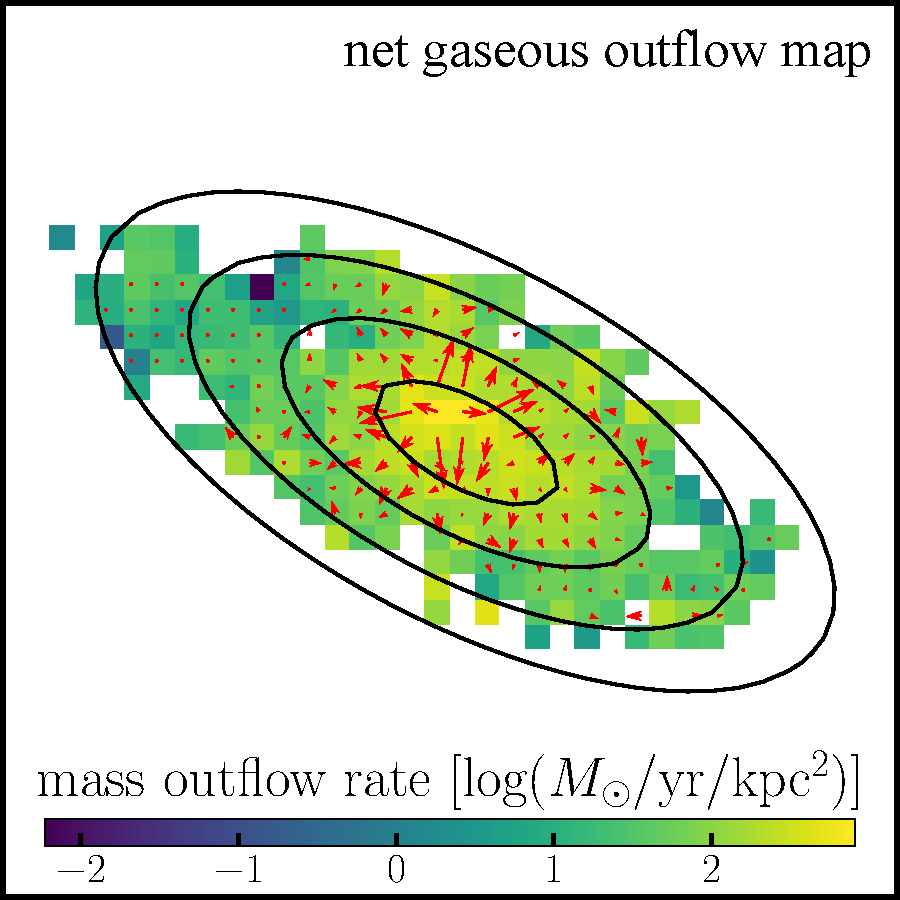
\includegraphics[width=.5\textwidth]{fig/outmass_ID03751.pdf}
    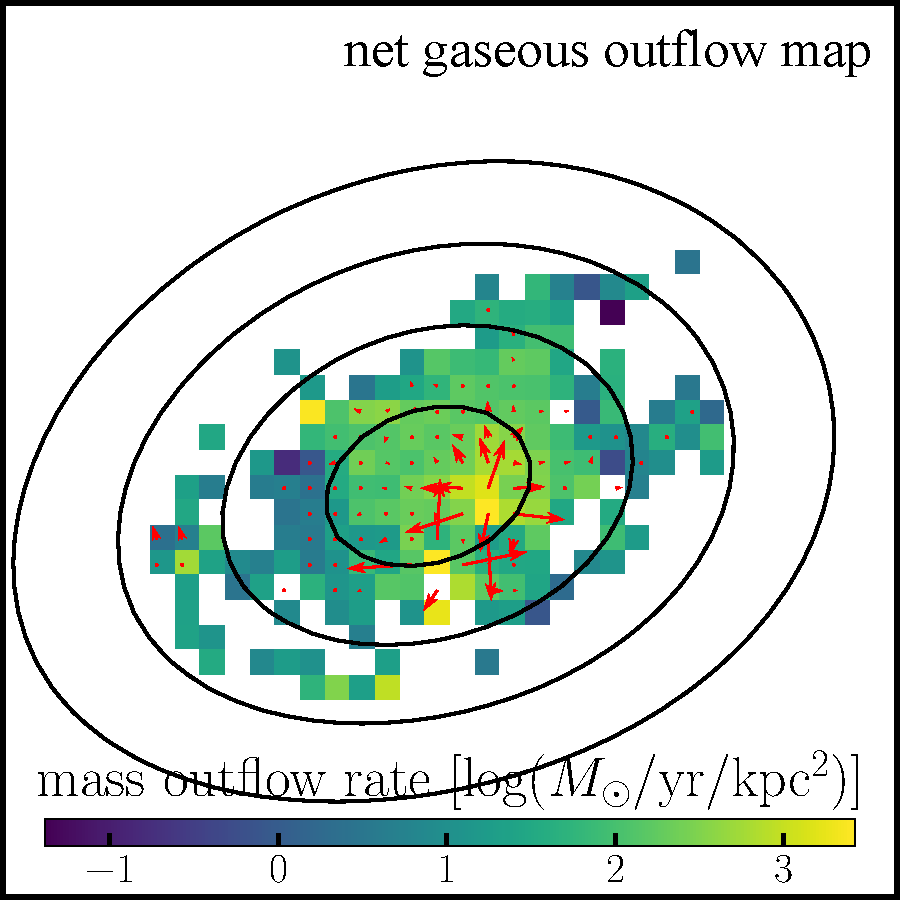
\includegraphics[width=.5\textwidth]{fig/outmass_ID01203.pdf}
    \caption[First ever maps of gaseous outflow rates at $z$$\sim$2.]
    {Maps of gaseous outflow rates derived from our analysis combining gas regulator models and empirical star-formation laws.
    The spatial extent and orientation follows that in Figure~\ref{fig:combELmap}.
    Red arrows show the net direction and magnitude of the gaseous outflows driven by galactic winds.
    We argue that outflows play a key role in effectively transporting stellar nucleosynthesis yields from the inner regions of 
    these two galaxies to their outskirts.
    \label{fig:outmass}}
\end{figure}
%= = = = = = = = = = = = = = = = = = = = = = = = = = = = = = = = = = = = = = = =

The application of simple chemical evolution in Section~\ref{sect:physprop} is enlightening but depends on 
strong assumption, such as that the azimuthal variations are negligible and galaxies live in equilibrium.
In reality, these conditions might not be valid, \eg, due to rapid gas flows.
To gain a more precise understanding of the physics of galactic winds and the role of gaseous outflows in 
shaping the observed spatial distribution of metallicity, independent of those assumptions, we can turn to a
more advanced framework for galaxy chemical evolution: the gas regulator model 
\citep{Lilly:2013ko,Peng:2014hn}.
This model provides an informative and coherent view of the full baryon cycle, involving the accretion of underlying DM halos, as 
well as the instantaneous regulation of star formation by a time-variable gas reservoir.
A key feature of this model is that it does not assume that galaxies live in an equilibrium state, where the total amount of gas 
mass remains constant. The non-equilibrium flexibility is especially important for applying this model to spatially resolved 
regions within a galaxy, where gas may be transported radially from one region to another. Chemical evolution within the gas 
regulator model is described by the equations
\begin{align}
    Z_{\rm gas} & = \left[Z_0 +
    y\taueq\epsilon\(1-\exp(-\frac{t}{\taueq})\)\right]\left[1 -
    \exp(\frac{-t/\taueq}{1-\exp(-t/\taueq)})\right],      \\
    \tau_{\rm eq} & = \frac{1}{\epsilon\(1-R+\lambda\)}.    \non
\end{align}
Here we adopt the convention of symbols itemized in Table~1 of \citet{Peng:2014hn}:
\Zgas is the mass fraction of metals in the gas reservoir (determined from the observed \oh as in \citet{Peeples:2011ew}), $t$ is 
the average stellar population age, $\taueq$ is the time scale on which the baryon cycle reaches equilibrium, $\epsilon$ is the 
\sf efficiency (defined as $\epsilon\equiv\SFR/\Mgas=\Sigma_\SFR/\Sgas$), and $\lambda$ is the mass loading factor (defined in 
terms of the mass outflow rate $\Psi$, such that $\lambda=\Psi/\SFR$\footnote{Note that $\lambda$ and $f_o$ in 
Section~\ref{sect:physprop} represent the same quantity but here we are solving for $\lambda$ in a spatially resolved fashion.}).
We adopt a stellar nucleosynthesis yield $y=0.003$ \citep{Dalcanton:2007kc} with $R=0.4$ estimated from BC03 
\citep{Bruzual:2003ck} stellar population models. Finally, we assume that gas inflows are pristine ($Z_0=0$).

For each spatial region where we have estimated the metallicity, \SFR, gas surface density, and age (Figures~\ref{fig:oh12grad}, 
\ref{fig:physmap}), we solve the above equations for the mass loading factor $\lambda$ and subsequently calculate the mass outflow 
rate $\Psi$.
The 2D distribution of $\Psi$ is displayed in Figure~\ref{fig:outmass}.
Taking the gradient field of this gaseous outflow map, we obtain the net direction of the outflowing mass flux on 
sub-galactic scales, projected along the line of sight, denoted by the red arrows in Figure~\ref{fig:outmass}.
The results demonstrate that strong galactic winds transport mass from the center to the outskirts, with the net 
radial transport of heavy elements causing the inverted gradients observed in our targets.

%= = = = = = = = = = = = = = = = = = = = = = = = = = = = = = = = = = = = = = = =
%%% Figure:
\begin{figure}
    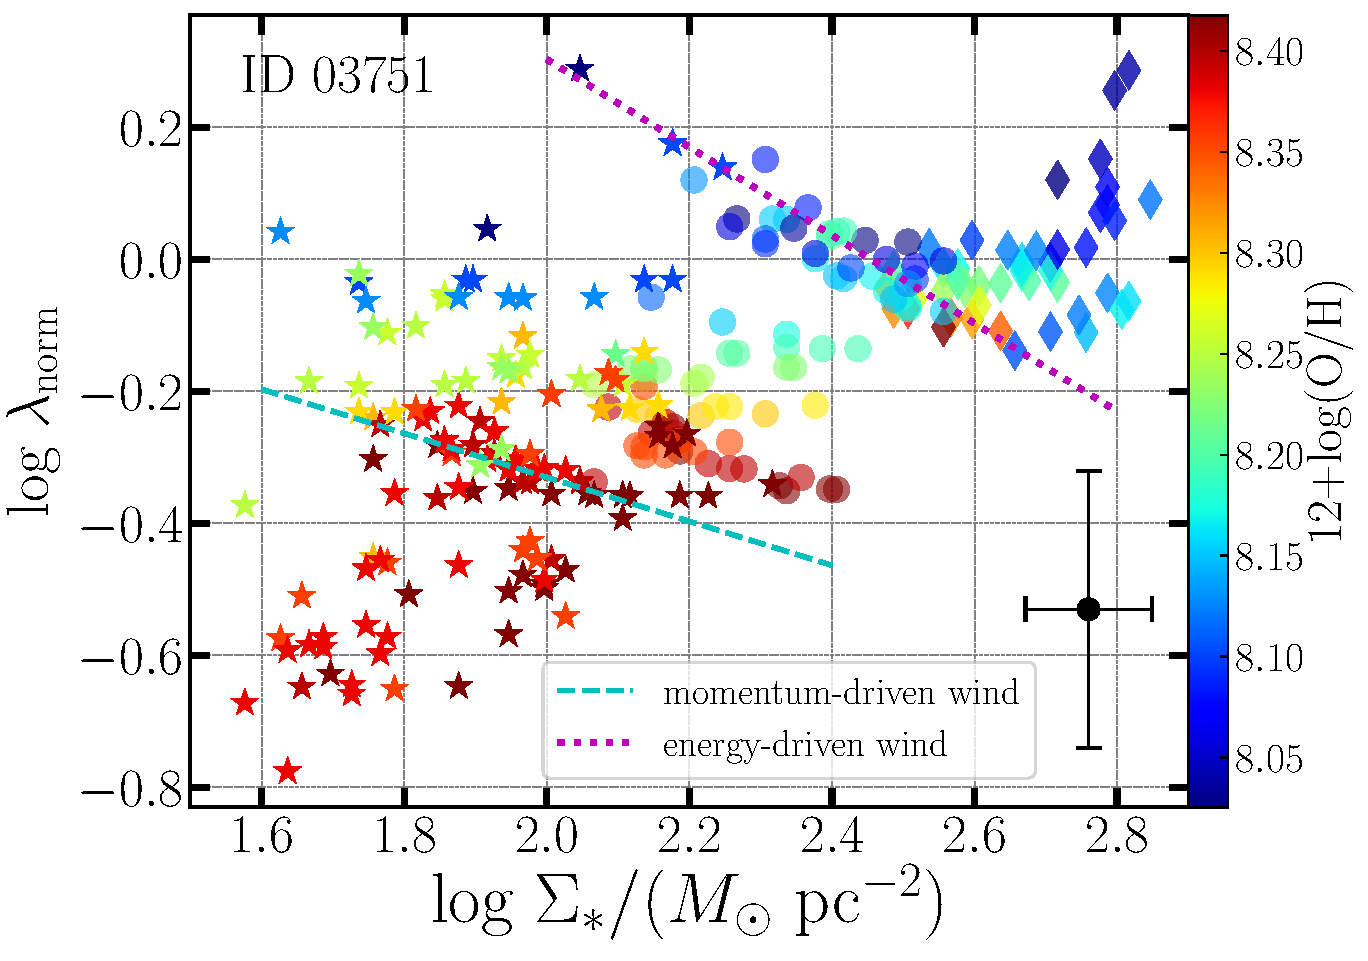
\includegraphics[width=.5\textwidth]{fig/lamSDstar_ID03751.pdf}
    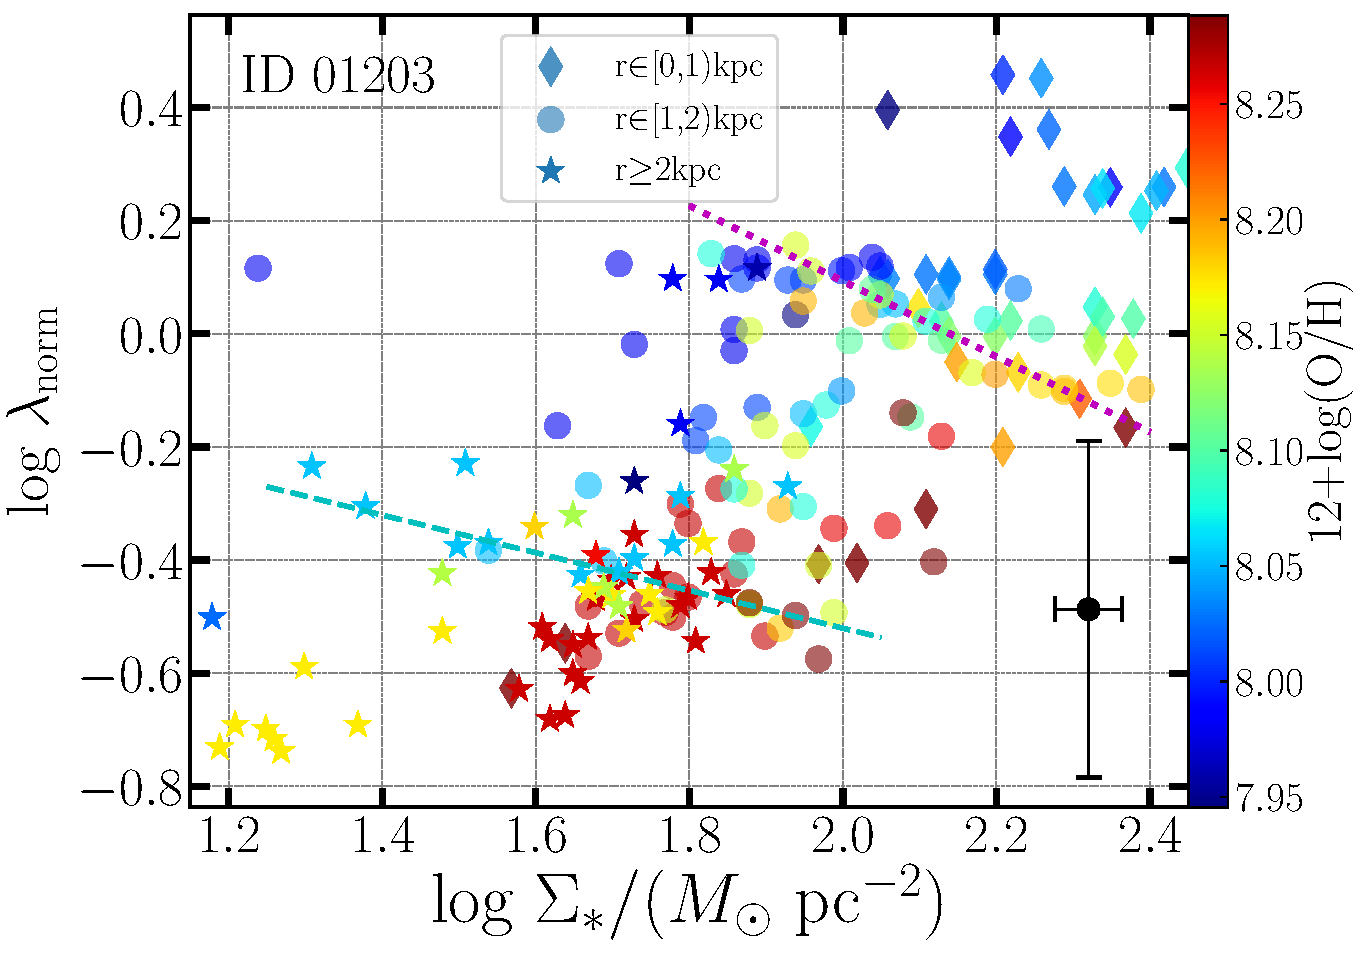
\includegraphics[width=.5\textwidth]{fig/lamSDstar_ID01203.pdf}
    \caption[Correlation between spatially resolved mass loading factor and stellar surface density.]
    {Correlation between spatially resolved mass loading factor $\lambda$ (normalized to the value at radius 1
    kpc; see Table~\ref{tab:srcprop}) and stellar surface density $\Sigma_\ast$, color-coded by metallicity.
    As in Figure~\ref{fig:physmap}, the diamond, circle, and star symbols represent measurements derived at a 
    galacto-centric radius
    of $r\in[0,1)$\kpc, $r\in[1,2)$\kpc, and $r\gtrsim2$\kpc, respectively.
    We overlay as an illustration two scaling relations that are commonly assumed to describe integrated measurements:
    $\lambda\propto\Sigma_\ast^{-2/3}$ for an energy-driven wind model marked by magenta dotted lines, and
    $\lambda\propto\Sigma_\ast^{-1/3}$ for a momentum-driven wind model by cyan dashed lines.
    Evidently, a single scaling relation is not sufficient to describe the spatially resolved data, demonstrating the need for a
    more sophisticated approach.
    The black point in the lower right corner in each panel displays the median uncertainties for these measurements.
    \label{fig:lamSDstar}}
\end{figure}
%= = = = = = = = = = = = = = = = = = = = = = = = = = = = = = = = = = = = = = = =

The distribution of mass loading factors $\lambda$ within each of our targets is also shown in 
Figure~\ref{fig:lamSDstar}, revealing higher $\lambda$ (and therefore a higher fraction of metals lost) in the central regions.
This preferential removal of metals from the center, and subsequent deposition at larger radii, gives rise to the strong 
positively sloped metallicity gradients evident in Figure~\ref{fig:oh12grad}.
The high values of $\lambda$ have important implications for the role of feedback in galaxy formation.
Most fundamentally, our results support feedback as a solution to the ``over-cooling'' problem in galaxy formation, by ejecting
gas and preventing overly condensed baryonic regions at high redshifts \citep{1978MNRAS.183..341W,Dekel:1986cv}.
Such strong outflows are also expected to suppress the formation of stellar bulges from low angular momentum gas 
\citep{Governato:2010ed,Brook:2012gj}.
This is consistent with low bulge fraction in these two galaxies measured from high resolution \hst imaging 
(Table~\ref{tab:srcprop}).

%A tantalizing feature in the $\lambda$ distribution is the co-existence of multiple wind modes {\em within} individual galaxies.
A key feature in the $\lambda$ distribution is that neither of the wind modes, driven by momentum or energy conservation, can 
explain the behavior of the mass dependence of $\lambda$ alone, {\em within} individual galaxies.
Outflows are typically parameterized by either a momentum-driven \citep{Oppenheimer:2006eq,Oppenheimer:2008bu} or an
energy-driven \citep{Springel:2003eg} wind mode, both of which are physically well motivated \citep{Murray:2005jt}.
The energy-driven wind scenario assumes that outflows are launched by the thermal pressure of supernova (SN) explosions and/or
winds from massive stars.
A portion of this thermal energy provides the outflow kinetic energy, \ie, $\Psi\times v^2_{\rm wind} \sim \SFR$, where the wind 
speed $v_{\rm wind}$ can mimic the escape velocity from DM halo, \ie, $v_{\rm esc}\sim M_{\rm h}^{1/3}$ given by the virial 
theorem.
This results in the scaling relation of $\lambda\propto\Mstar^{-2/3}$, assuming the linear correlation between the mass 
constituents of stellar and dark components.
The energy-driven wind model is found successful in explaining the low abundance of satellite galaxies in the Milky Way 
\citep{Okamoto:2010ba}.
The momentum-driven wind model instead relies on the momentum injection deposited by radiation pressure from SN explosions and/or 
massive stars, leading to $\Psi\times v_{\rm wind} \sim \SFR$ and $\lambda\propto\Mstar^{-1/3}$.
In this scenario, $v_{\rm wind}$ is proportional to \Mstar and \SFR, broadly consistent with some observational
results \citep{Martin:2005kx}.
The transition from energy- to momentum-driven winds is typically thought to be a galaxy-wide phenomenon,
resulting in the steepening of the mass-metallicity relation below \Mstar~$\simeq10^{9.3}$\Msun at $z\simeq2$ 
\citep{Henry:2013gx}.
However, our analysis indicates that a single mode is not sufficient to describe spatially resolved data \emph{within} one galaxy 
and it is highly likely that the transition from energy- to momentum-driven winds occurs on sub-galactic scales, governed by local 
gas and star formation properties in addition to the global gravitational potential.
%Specifically the data in the central region appear to cluster around the more powerful energy-driven scaling, while the outskirts 
%are roughly in the region covered by the scaling for a momentum-driven wind.


\section{Summary and Discussion}\label{sect:conclu}

We present the first robust confirmation of the existence of strongly inverted metallicity radial gradient (\ie $\gtrsim$0.1 
dex/kpc) in star-forming dwarf galaxies ($\Mstar\lesssim10^9\Msun$) at the peak of star formation and chemical enrichment 
($z\sim2$).
Our synergy of the diffraction-limited imaging spectroscopy from \hst NIR grisms and lensing magnification permits exquisite 
spatial sampling, \ie, at the scale of 50-100 pc, to securely resolve our $z\sim2$ galaxies with $\gtrsim$300 resolution elements 
(Figures~\ref{fig:combELmap} and \ref{fig:oh12grad}) to deliver precise radial gradient measurements.
To understand the physical origin of these strongly inverted gradients, we obtain high resolution 2D maps of star formation rate, 
characteristic stellar age (or equivalently star formation timescale), and gas fraction, from \hst observations of source stellar 
continuum and nebular emission.
These 2D maps show that the galactic disks of our sources are rapidly assembling stellar mass through in-situ star formation, in 
the early phase of inside-out growth (Figure~\ref{fig:physmap}).
By comparing our observations with simple chemical evolution models, we find that gas accretion alone cannot explain these 
strongly inverted gradients in our galaxies (Figures~\ref{fig:Zerb_fgas}).

Using a more advanced gas regulator model, we are able to calculate the spatial distribution of mass loss rates from outflows, 
treating each spaxel as an independent star-forming region, and thus map the macroscopic patterns of net gaseous outflows 
(Figure~\ref{fig:outmass}).
It turns out that the mass loss rates are highest in the central regions of both galaxies, coincident with
the peak star formation surface densities.
A natural explanation is thus that active star formation in galaxy centers gives rise to powerful winds that transport gas and
metals away from the center toward larger radii, forming ``galactic fountains'' \citep{Martin:2002ee}.

Furthermore, our spatially resolved analysis of metals, \SFR, and stellar populations shows that a single type of wind mechanism 
(either energy or momentum driven) cannot explain the entire galaxy (Figure~\ref{fig:lamSDstar}).
A primary physical parameter that has been proposed to set the transition between the two wind dynamics is the gravitational 
potential, often parameterized by velocity dispersion ($\sigma$). There exists a critical scale \scrit 
\citep{Murray:2005jt} such that for galaxies with $\sigma<\scrit$, energy injection by SNe sets a limiting 
\SFR above which interstellar gas is ejected in galactic winds. For galaxies with $\sigma>\scrit$, momentum 
deposition limits the maximum \SFR above which the ISM is likewise ejected.
The presence of both energy- and momentum-driven wind scalings in one galaxy suggests that feedback-triggered winds are connected
to physical properties on sub-galactic scales, \eg, \emph{local} velocity dispersion ($\sigma_{\rm local}$), 
which is sensitive to the optical depth of gas flows, the coupling efficiency between gas clouds and dust 
parcels, \etc.
On sub-galactic scales, there exists a strong correlation among velocity dispersion (not necessarily 
$\sigma_{\rm local}$), surface density and size of molecular clouds \cite[see][and references 
therein]{BallesterosParedes:2011gk}.
It appears that in our galaxies, the wind-launching mechanism transitions from energy- to momentum-driven as 
galacto-centric radius increases.
This gives rise to a hypothesis that $\sigma_{\rm local}$ in our galaxies should increase from inner to outer 
regions.
%straddling a critical value similarly defined as $\scrit$.
Our current kinematic data on source ID 01203 have high spatial resolution (at $0\farcs05$ plate scale) yet narrow FoV so that it 
is infeasible to map sub-kpc scale velocity dispersion accurately to outer regions at $r\gtrsim2$ \kpc, where momentum-driven wind 
seems to take over.
To test this hypothesis conclusively, more spatially resolved data taken under sufficient spatial sampling will be required to 
robustly derive a full 2D map of velocity dispersion out to the periphery of the galactic disk, using instruments 
with relatively large FoV, \eg, the \jwst NIRSpec IFU \citep{Kalirai:2018gs}.

Physically, the momentum-driven wind scaling applies to ``cool'' ($T \sim 10^4$ K) ambient interstellar gas entrained in outflows,
whereas the energy-driven wind is appropriate when entrained gas is shock heated to temperatures where cooling is inefficient ($T
\sim 10^6$ K). A plausible scenario for our galaxies is that feedback from an intense burst of star formation in the central
regions heats the ejected gas to a highly ionized phase, while gas entrained in outflows from the outer regions remains cool. If
this interpretation is correct, then we expect a distinct signature in the absorption properties of outflowing gas. Outflows from
the central regions should be dominated by highly ionized species (e.g. \ionp{O}{vi}, \ionp{C}{iv}, \ionp{Si}{iv}) whereas
outflows from the outer regions should have relatively more of the low ions characteristic of $T \sim 10^4$ K gas (e.g.
\ionp{Fe}{ii}, \ionp{Mg}{ii}, \ionp{Si}{ii}). Both high and low ion species are commonly observed in outflows from star forming
galaxies at $z\simeq2$ \citep{Berg:2018gd,Du:2018tr}, although their spatial distributions are not yet well known 
\citep[but see][]{James:2018km}.
Our hypothesis suggests a more central concentration of the high ions \emph{in the specific cases} where a 
combination of both outflow scalings results in inverted metallicity gradients.
This prediction can be directly tested with spatially resolved spectroscopy of rest-frame
ultraviolet absorption lines using instruments such as \keck/KCWI or VLT/MUSE.


\renewcommand{\thesection}{\thechapter.A}
\section{Appendix}

\renewcommand{\thesubsection}{\thechapter.A.\arabic{subsection}}
\subsection{Gas kinematics from \keck \osiris observations}\label{sect:kinem}

Kinematics of \HII regions are of interest both for determining whether rotating gaseous disks are present, and the overall scale 
of velocity dispersion which is thought to correlate with the mode of feedback.  We have obtained kinematic maps from \Ha emission 
for source ID 01203 as part of a GLASS followup campaign with the \osiris integral field spectrograph 
\citep{Larkin:2006jd} on the \keck I telescope. Full details of the observations and analysis are presented 
elsewhere \citep{Hirtenstein:2018tn}; here we give a brief summary.  Data were obtained on 2016 October 21 using 
the Hn5 filter, 50 milliarcsecond scale, and laser guide star AO, which provides the excellent spatial sampling 
needed to resolve velocity structure on the relevant $\sim$0\farcs1 scales. We obtained 3 exposures of 900 
seconds each.  The \osiris Data Reduction Pipeline was used to process the data, following the standard methods 
adopted in our previous work \citep{2013ApJ...765...48J}. We fit \Ha line emission in each spaxel with a Gaussian 
function, requiring $\geq5\sigma$ significance for acceptable fits. Gas rotation velocity ($V$) and velocity 
dispersion ($\sigma$) are determined from the Gaussian centroid and width. We correct velocity dispersions for 
the effects of instrument resolution and beam smearing by subtracting these terms in quadrature from the best-fit 
Gaussian dispersion. The median beam smearing correction is a 7\% reduction in $\sigma$. 

Resulting maps of $V$ and $\sigma$ in Figure~\ref{fig:kinem} reveal a sheared velocity field with high local velocity dispersion
($\gtrsim50$ \kms), common among disk galaxies at similar redshift. To quantify the degree of rotational support, we extract a 1D
velocity profile along the kinematic major axis. We fit this with the circular rotation curve of an exponential
disk mass profile. The disk rotation curve is in good agreement with the data, with maximum velocity $V\sin i = 94\pm7$ \kms.
Here $i$ is the disk inclination angle relative to the line-of-sight. The pixel-averaged $\sigma = 73\pm3$ \kms 
such that we derive $V/\sigma = (1.3\pm0.1) / \sin i$ indicating orderly rotation in spite of a high level of ISM 
turbulence.
This $V/\sigma$ ratio is typical of the galaxy population harboring thick disks
at similar mass and redshift \citep{2015ApJ...799..209W,2015arXiv150901279L}.

%= = = = = = = = = = = = = = = = = = = = = = = = = = = = = = = = = = = = = = = =
%%% Figure: kinematic plots for ID 01203
\begin{figure}
    \centering
    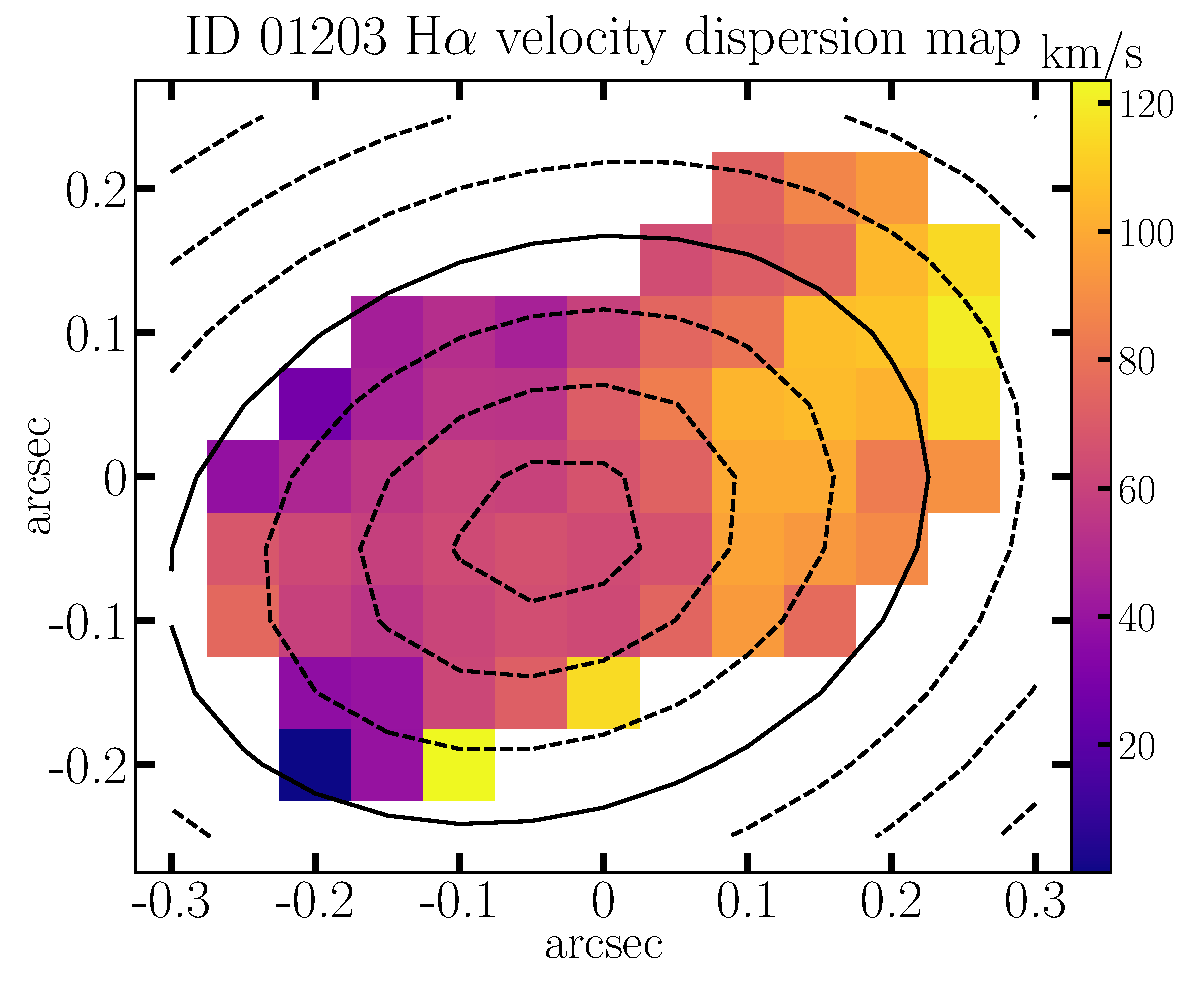
\includegraphics[height=1.7in]{fig/dispersion_ID01203.pdf}
    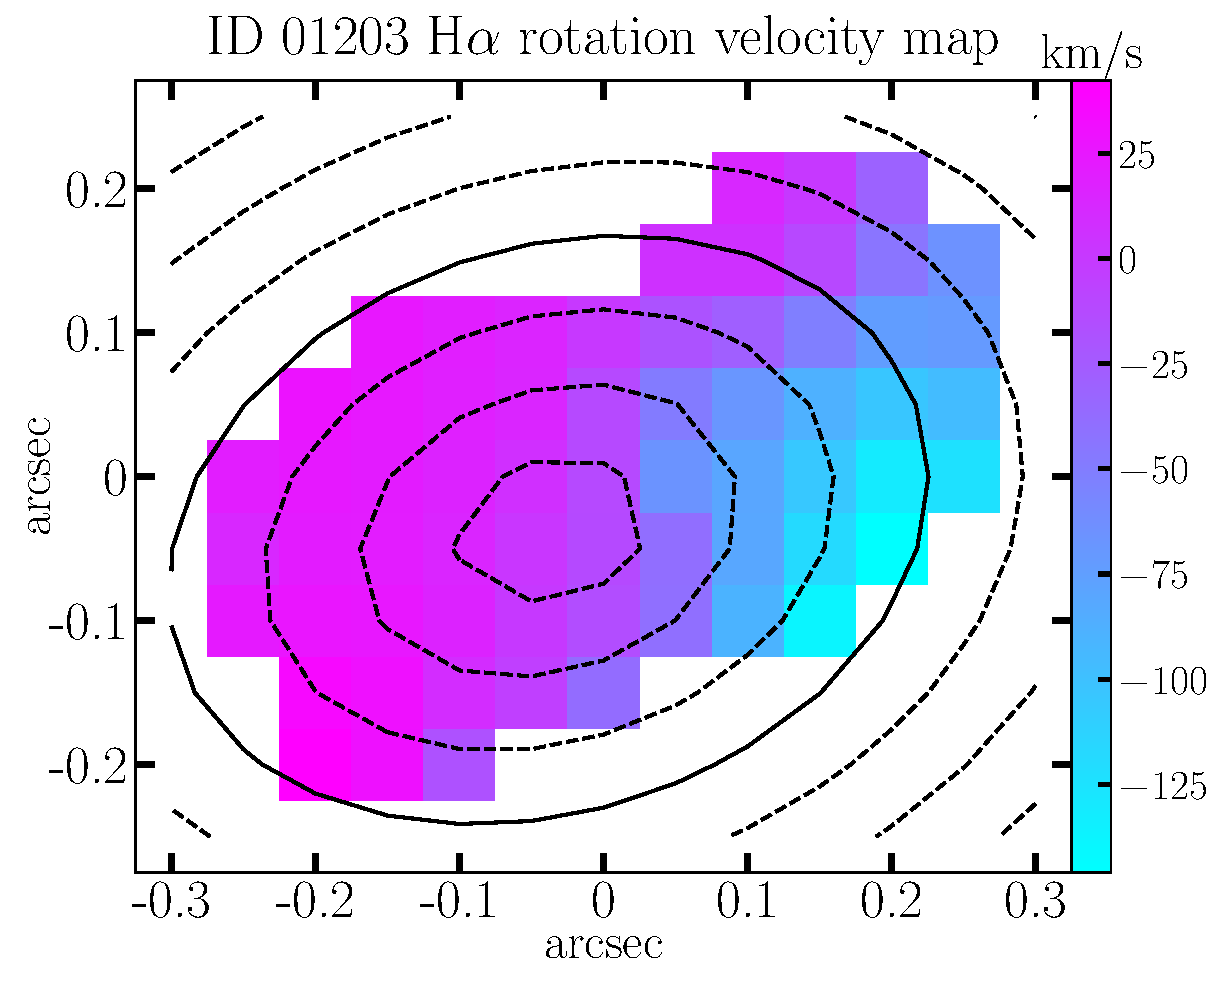
\includegraphics[height=1.7in]{fig/rotation_ID01203.pdf}
    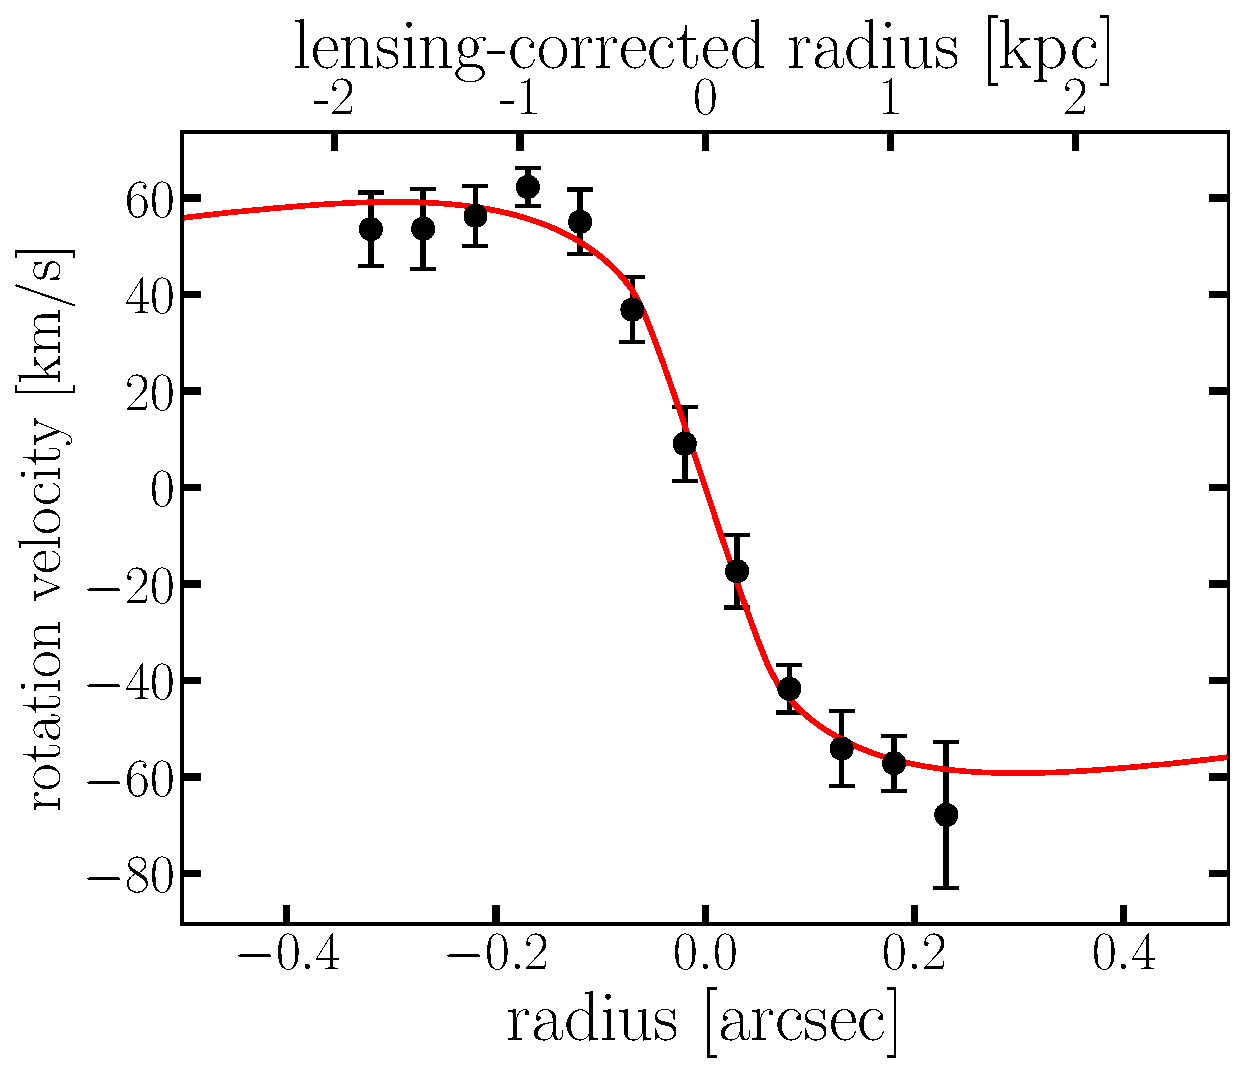
\includegraphics[height=1.7in]{fig/rotcurve_ID01203.pdf}
    \caption[\Ha emission kinematics of ID 01203 from our \osiris AO-assisted observations.]
    {\Ha emission kinematics of ID 01203 from our \osiris AO-assisted observations showing the velocity 
    dispersion ({\it
    left}), the rotation velocity ({\it center}), and rotation curve extracted along the major axis ({\it right}).
    The overlaid contours in the left and center panels also represent the source plane de-projected galacto-centric radii, but in
    0.25 kpc interval. To give relative scale with respect to our \hst stamps, the 1 kpc radius contour is still in solid.
    The red curve in the right panel is the best-fit rotation curve for an exponential disk mass distribution, giving a maximum
    line-of-sight velocity $V\sin i = 94 \pm 7$ \kms.
    The data are in good agreement with a thick disk rotation curve despite a high level of turbulence.
    \label{fig:kinem}}
\end{figure}
%= = = = = = = = = = = = = = = = = = = = = = = = = = = = = = = = = = = = = = = =


\renewcommand{\thesubsection}{\thechapter.A.\arabic{subsection}}
\subsection{Extracting and fitting 1D and 2D \protect\hst grism spectra}\label{sect:grismspec}

As briefly mentioned in Section~\ref{subsect:grism_reduce}, we employed the Grism Redshift and Line analysis 
software \grzl to reduce the \hst WFC3/NIR grism data from raw exposures acquired by the \glass program.
Our primary goal is to obtain the spatially resolved emission line intensities after removing the contribution 
from source continuum.
In terms of modeling the continuum spectrum, \grzl first produces a simple flat (in $F_{\lambda}$)
spectral model for all sources within the WFC3 FoV with \H-band magnitude brighter than 26 ABmag.
The normalization is determined to match the flux in the corresponding reference image (in our cases, F105W as 
the reference to G102, and F140W to G141, ascribed to similar wavelength coverage).
Then second-order polynomial functions are fitted to the sources whose \H-band magnitude is brighter than 24 
ABmag.
This process is done iteratively, until a convergence point where the residual in the grism exposures after
subtracting the fitted continuum models becomes negligible.

While the polynomially fitted continuua serve as good enough models for contamination subtraction
associated with neighboring objects, this polynomial functional form is clearly not physically representative of
the actual SED of the underlying stellar continuum for our sources of interest.
To facilitate a more accurate continuum subtraction, we further refine the source continuum model by considering 
primarily four template continuum spectra in a range of characteristic ages for stellar populations:
\begin{enumerate}
    \item a low-metallicity Lyman-break galaxy (Q2343-BX418) showing very young, blue continuum 
    \citep{Erb:2010iy},
    \item an intermediate-age composite SED with moderate Balmer break and 4000 \AA{} break, synthesized in 
    \citet{Brammer:2008gn} following the method of \citet{KCorrectionsandFi:WJFCKqrW},
    \item a post-starburst SED showing prominent Balmer break and 4000 \AA{} break from the UltraVISTA survey 
    \citep{Muzzin:2013is},
    \item a single stellar population SED with a 13.5 Gyr age and solar metallicity \citep{Conroy:2012bl}.
\end{enumerate}
This combination of both empirical and synthetic SED templates constitutes an optimized set appropriate for 
redshift fitting and continuum subtraction under our situation.
As discussed in \citet{Brammer:2008gn}, there is a trade-off between the number of templates used in SED fitting 
and numerical efficiency, and they find that the improvement is negligible if the number of templates is 
increased to above 5.
For a sanity check, we also run the template fitting procedures using a more complete template library built from 
the Flexible Stellar Population Synthesis (FSPS) models \citep{Conroy:2009ks,Conroy:2010ja,Conroy:2010bi} and 
found no noticeable changes in the spectroscopic redshift determinations nor continuum subtractions.

In addition to fitting stellar continuum, we model the intrinsic nebular emission lines in 1D spectra as Gaussian
functions. The amplitudes and flux ratios between most of the line species are allowed to vary (except for some
certain line complexes, \eg, $f_{\OIII~5008}/f_{\OIII~4960}$ = 3:1).
Given the relatively low instrument resolution of \hst grisms, the dynamic motion of gas and stellar components 
leave no effect on the observed profiles (both in 1D and 2D) of line emission/absorption features.
However, for spatially extended sources, the effective spectral resolution is lowered by morphological broadening 
\citep{vanDokkum:2011cq}, which usually varies with respective to the light-dispersion direction, \ie, the 
position angle (P.A.).
We explicitly take the source morphology into account via convolving the model spectra (stellar continuum + 
nebular emission) with the direct image in reference frames averaged along light-dispersion directions.

As a result, in Figures~\ref{fig:3751spec} and \ref{fig:1203spec}, we show the observed and fitted grism spectra 
for both of our sources at separate P.A.s.
Albeit slightly different in shape and slope, the red curves in 1D spectra comes from the same best-fit spectral 
model for each source and the difference is due to slightly varying morphological broadening.
We also see that the 2D continuum-subtracted spectra are sufficiently clean, preserving only the nebular emission
features that we later combined to get the spatially resolved emission line maps shown in 
Figure~\ref{fig:combELmap}.

\begin{figure}
    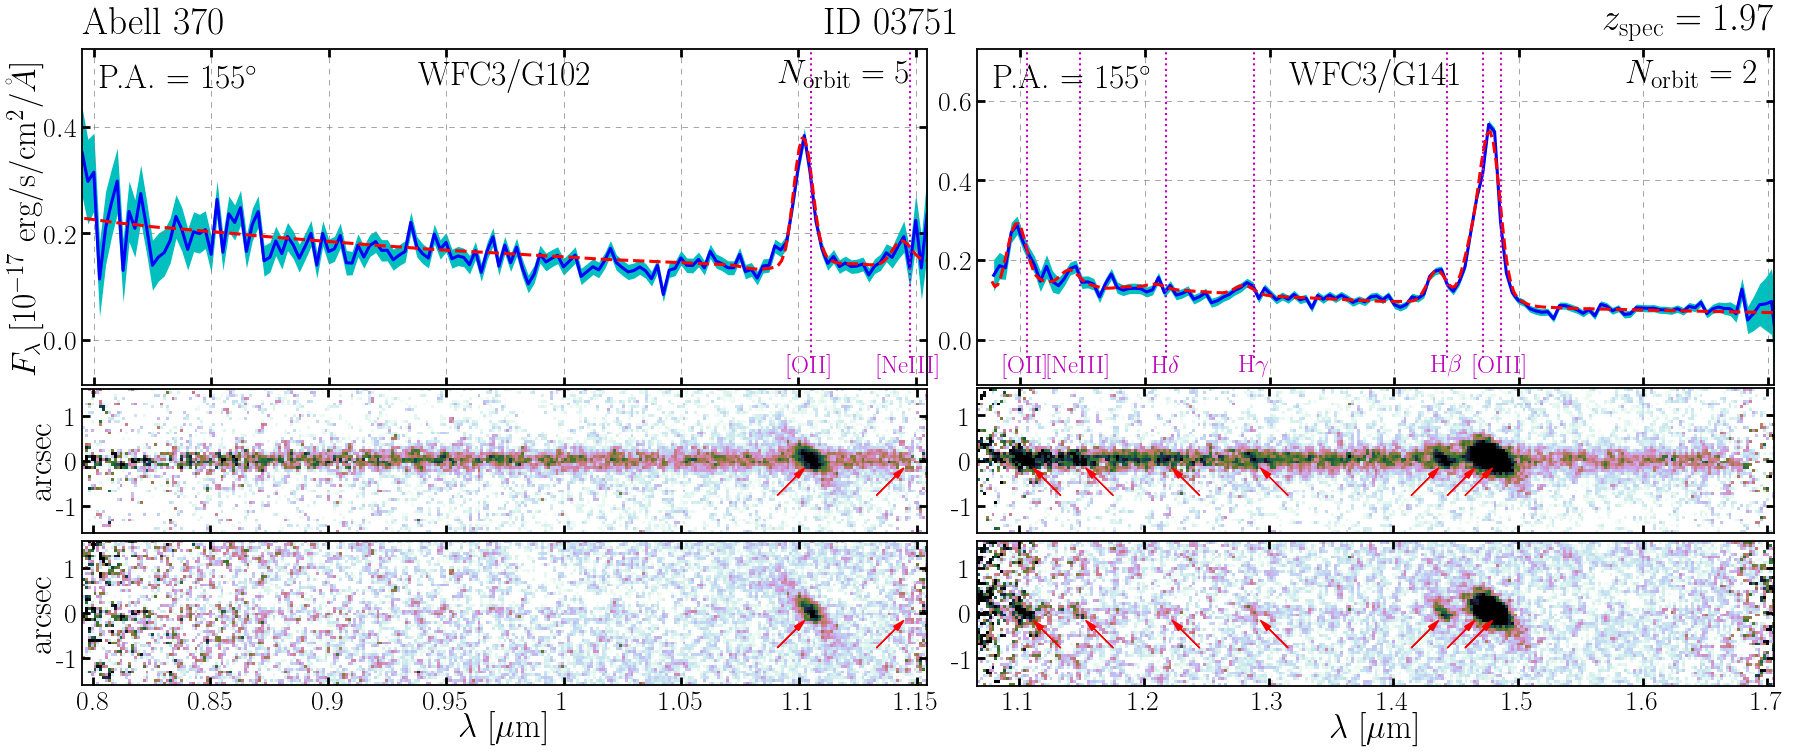
\includegraphics[width=\textwidth]{fig/clA370_id03751_pa155_ELfig.png}
    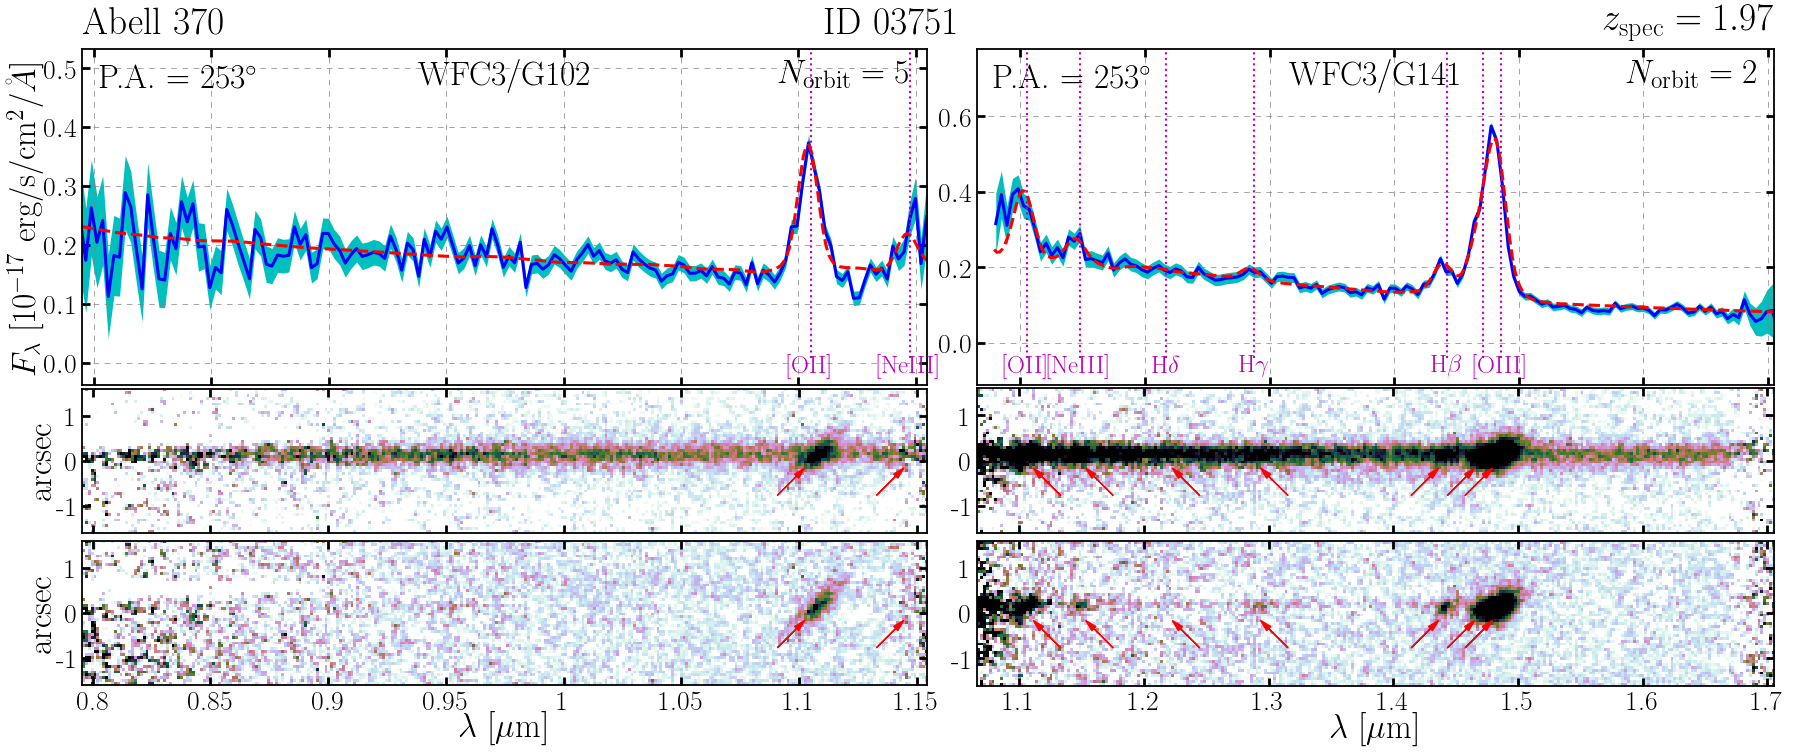
\includegraphics[width=\textwidth]{fig/clA370_id03751_pa253_ELfig.png}
    \caption[The \hst grism spectra for source ID 03751 in the field of \clsan taken by the \glass program.]
    {The \hst grism spectra for source ID 03751 in the field of \clsan taken by the \glass program.
    The total science integration is equally distributed into two separate P.A.s,
    reaching 5 orbits of G102 exposures and 2 orbits of G141 exposures per P.A., shown in two sub-figures.
    In each sub-figure, from top to bottom, we show the optimally extracted 1D spectra and the full 2D spectra 
    before and after source continuum subtraction, for both grism elements.
    On the 1D spectra, the observed flux is represented by the blue solid line with 1-$\sigma$ noise level 
    denoted by the cyan shaded band, and the 1D model spectrum (source continuum + nebular emission) is 
    represented by the red dashed curve.
    The observed locations of emission features are highlighted by vertical dotted lines in magenta and arrows in 
    red, in 1D and 2D spectra respectively.
    }
    \label{fig:3751spec}
\end{figure}

\begin{figure}
    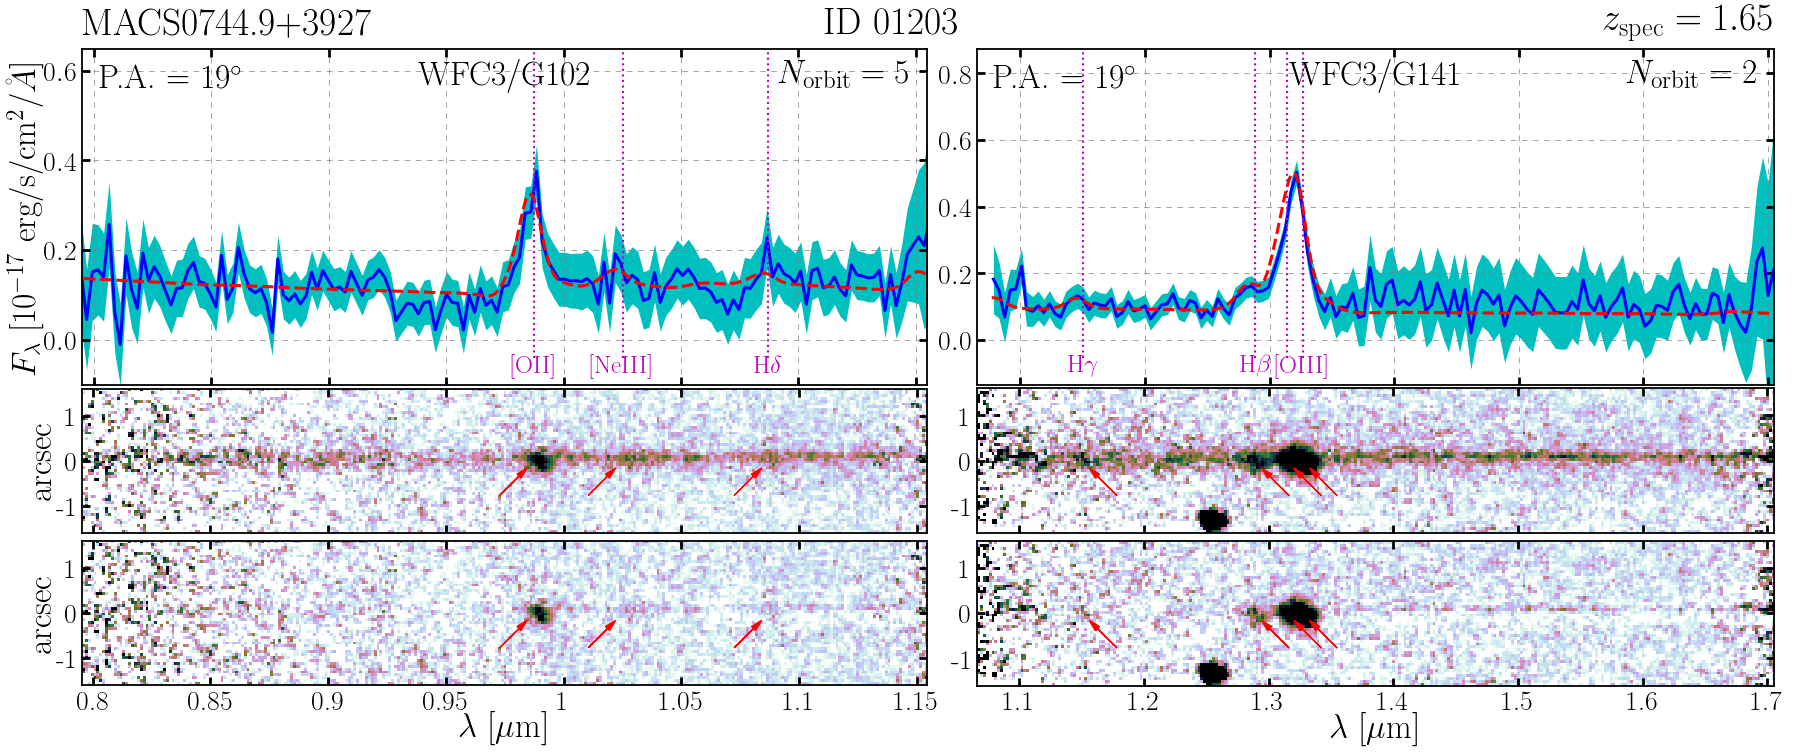
\includegraphics[width=\textwidth]{fig/clM0744_id01203_pa019_ELfig.png}
    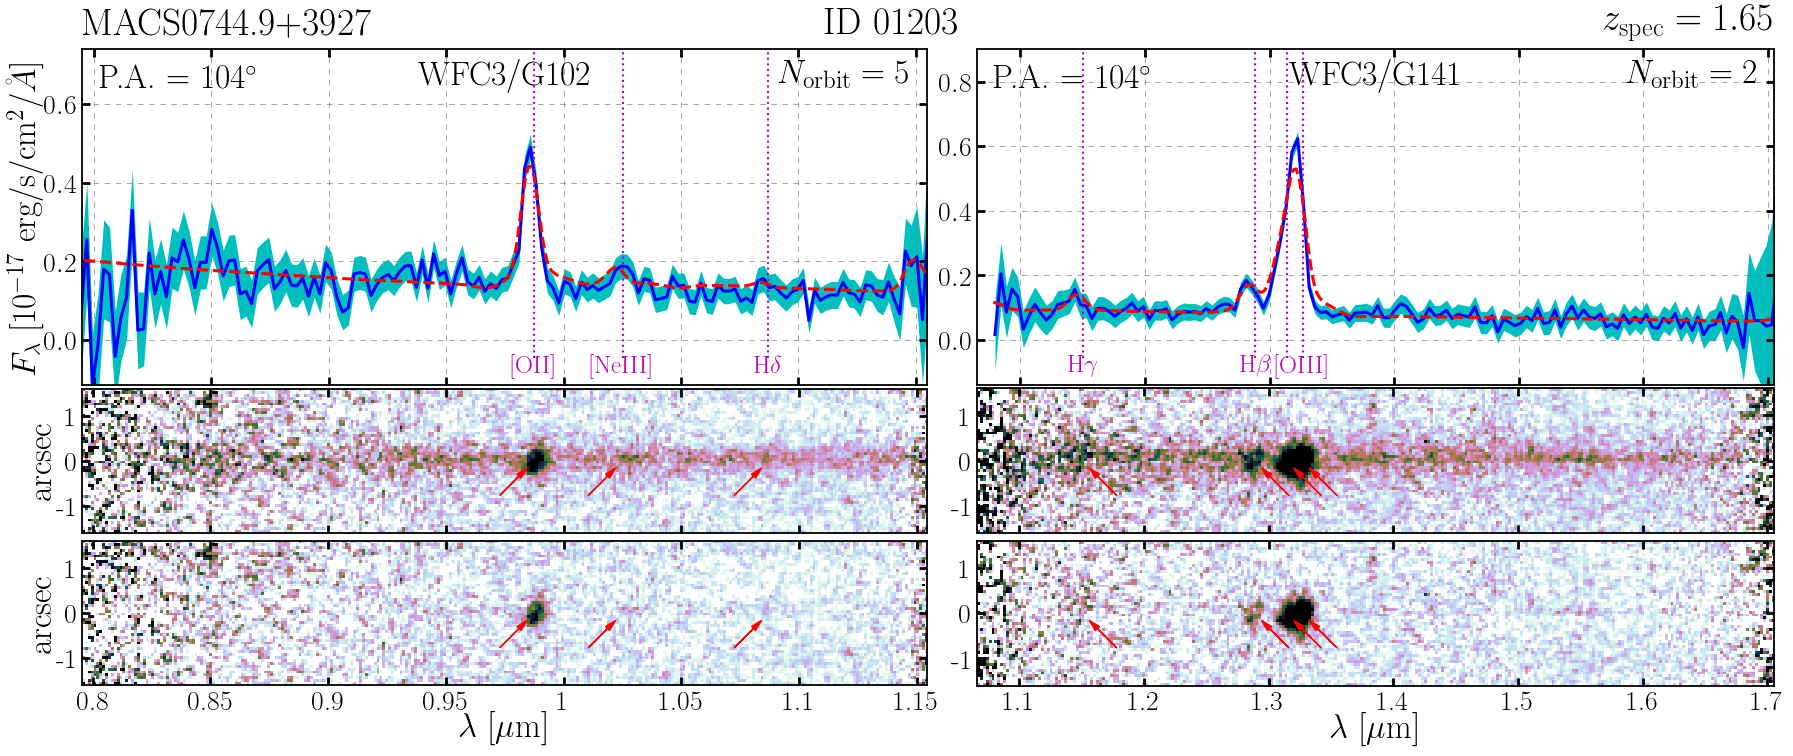
\includegraphics[width=\textwidth]{fig/clM0744_id01203_pa104_ELfig.png}
    \caption[Same as Figure~\ref{fig:3751spec}, except that source ID 01203 in the field of \clba is shown.]
    {Same as Figure~\ref{fig:3751spec}, except that source ID 01203 in the field of \clba is shown.}
    \label{fig:1203spec}
\end{figure}


